\documentclass[12pt]{article}
\usepackage{enumerate,amsmath,amssymb,mathrsfs,amscd,stmaryrd,amsthm}
\usepackage[margin=1.2in]{geometry}
%\usepackage{enumerate,amsmath,amssymb,mathrsfs,amscd,amsthm}
\usepackage{marvosym}
\usepackage{makeidx}
\usepackage{setspace}
\usepackage{graphicx}
\usepackage{color}
\usepackage[all]{xy}
\usepackage{tikz}
%\usepackage{url}
\usepackage[colorlinks=true,urlcolor=blue,linkcolor=black]{hyperref}
\usetikzlibrary{matrix,arrows}
%\onehalfspacing

\usepackage[mathcal]{euscript}

%\usepackage[colorinlistoftodos]{todonotes}

% RSF's exerersises style
%\usepackage{exers}

% -------  INCLUSION OF SOLUTIONS --------------------
\usepackage{ifthen}
\newboolean{includeSolutions}
%\setboolean{includeSolutions}{true}
\setboolean{includeSolutions}{false}
 
\raggedbottom

\theoremstyle{plain}
\newtheorem{theorem} {Theorem}
\newtheorem{corollary}[theorem]{Corollary}
\newtheorem*{main} {Main-Theorem}
\newtheorem{lemma}[theorem]{Lemma}
\newtheorem{prop}[theorem]{Proposition}
\theoremstyle{definition}
\newtheorem{definition}[theorem]{Definition}
\newtheorem{example}[theorem]{Example}
\newtheorem{examples}[theorem]{Example}
%\newtheorem{exercise}[theorem]{{\LARGE \Bicycle} Exercise}
%\newtheorem{exers}[theorem]{{\LARGE \Bicycle} Exercises}
\newtheorem{exercise}{Exercise}
\newtheorem{exers}[theorem]{Exercises}
\theoremstyle{remark}
\newtheorem*{notation}{Notation}
\theoremstyle{remark}
\newtheorem{remark}[theorem]{Remark}
%\newtheorem{problem}[theorem]{Problem}

% I temporarily commented out \usepackage{exers} (above) and added the next two
% lines so mine would compile even without the exers.sty file. 
%  \newtheorem{exercises}{Exercises}
%  \newtheorem{problem}[theorem]{Problem}

% [WJD] Suggestion: to begin a numbered list of examples, use
% \begin{examples}~
%   \begin{enumerate}[(a)]
%   \item  ...

%\numberwithin{definition}{section}
\numberwithin{theorem}{section}
%\numberwithin{corollary}{section}
%\numberwithin{prop}{section}
%\numberwithin{lemma}{section}
\numberwithin{equation}{section}


% For consistency, we should agree upon some special notation:
\newcommand{\cd}{\Crossedbox}  % contradiction
\newcommand{\<}{\ensuremath{\langle}}
\renewcommand{\>}{\ensuremath{\rangle}}

% SET THEORY & RELATIONS
% To specifiy that the symbol R is a binary relation use: x \rel{R} y
\newcommand{\rel}[1]{\ensuremath{\mathbin{#1}}}
\newcommand{\rR}{\ensuremath{\rel{R}}}  % or just x \rR y

\newcommand{\id}{\ensuremath{\operatorname{id}}}       % identity
\newcommand{\dom}{\ensuremath{\operatorname{dom}}}   % the domain of a relation
\newcommand{\fld}{\ensuremath{\operatorname{fld}}}   % the field of a relation
\newcommand{\ran}{\ensuremath{\operatorname{ran}}}   % the range of a relation
\newcommand{\card}{\ensuremath{\operatorname{card}}} % cardinality
\newcommand{\res}{\ensuremath{\upharpoonright}}  % restriction
\newcommand{\es}{\ensuremath{\varnothing}}
\renewcommand{\emptyset}{\ensuremath{\varnothing}}
\newcommand{\llb}{\ensuremath{\llbracket}}
\newcommand{\rrb}{\ensuremath{\rrbracket}}
\newcommand{\lb}{\ensuremath{[}}
\newcommand{\rb}{\ensuremath{]}}
\newcommand{\power}[1]{\ensuremath{\mathscr{P}(#1)}}  % power set

\newcommand{\gl}{\lambda}

% (slanted inequalities look much nicer than the standard ones)
\renewcommand{\leq}{\ensuremath{\leqslant}}   
\renewcommand{\nleq}{\ensuremath{\nleqslant}}
\renewcommand{\geq}{\ensuremath{\geqslant}}
\renewcommand{\ngeq}{\ensuremath{\ngeqslant}}

% ALGEBRAS
% An algebra should be written inside angled brackets:
\newcommand{\algebra}[1]{\ensuremath{\langle #1 \rangle}}
% Example:    \algebra{A; F}  -->  <A; F>
\newcommand{\Con}{\ensuremath{\operatorname{Con}}}
\newcommand{\bCon}{\ensuremath{\mathbf{Con}}}
\newcommand{\arity}{\ensuremath{\operatorname{arity}}}
\newcommand{\Sub}{\ensuremath{\operatorname{Sub}}}     % \Sub(A) = set of subalgebras of A
\newcommand{\bSub}{\ensuremath{\mathbf{Sub}}}    % \bSub A = lattice of subalgebras of A
\newcommand{\Sg}{\ensuremath{\operatorname{Sg}}}       % \Sg(X) = subalgebra generated by the set X
\newcommand{\Hom}{\ensuremath{\operatorname{Hom}}}     % homomorphisms
\newcommand{\Aut}{\ensuremath{\operatorname{Aut}}}     % automorphisms
\newcommand{\End}{\ensuremath{\operatorname{End}}}     % endomorphisms

% GROUPS
\newcommand{\GL}{\ensuremath{\operatorname{GL}}}
\newcommand{\PSL}{\ensuremath{\operatorname{PSL}}}
\newcommand{\Eq}{\ensuremath{\operatorname{Eq}}}
\newcommand{\bEq}{\ensuremath{\mathbf{Eq}}}
\newcommand{\core}{\ensuremath{\operatorname{core}}}
\newcommand{\subnormal}{\ensuremath{\trianglelefteqslant}}
\newcommand{\supnormal}{\ensuremath{\trianglerighteqslant}}
\newcommand{\notsubnormal}{\ensuremath{\ntrianglelefteqslant}}

\newcommand{\meet}{\ensuremath{\wedge}}
\newcommand{\two}{\ensuremath{\mathbf{2}}}
\newcommand{\join}{\ensuremath{\vee}}
\newcommand{\Meet}{\ensuremath{\bigwedge}}
\renewcommand{\Join}{\ensuremath{\bigvee}}
\newcommand{\lub}{\ensuremath{\operatorname{lub}}}
\newcommand{\glb}{\ensuremath{\operatorname{glb}}}
\newcommand{\Sym}{\ensuremath{\operatorname{Sym}}}

% FIELDS
\newcommand{\ch}[1]{\text{char}(#1)}


% NAMES
\newcommand{\Tuma}{T\r{u}ma}
\newcommand{\Palfy}{P\'alfy}
\newcommand{\Pudlak}{Pudl\'ak}

\newcommand{\ex}{\marginpar[{\LARGE \Bicycle}]{{\LARGE \Bicycle}}}

% FONT SHORTCUTS
\newcommand{\bA}{\ensuremath{\mathbf{A}}}
\newcommand{\bB}{\ensuremath{\mathbf{B}}}
\newcommand{\bY}{\ensuremath{\mathbf{Y}}}
\newcommand{\bG}{\ensuremath{\mathbf{G}}}
\newcommand{\bM}{\ensuremath{\mathbf{M}}}
\newcommand{\bF}{\ensuremath{\mathbf{F}}}
\newcommand{\bE}{\ensuremath{\mathbf{E}}}
\newcommand{\bR}{\ensuremath{\mathbf{R}}}

\newcommand{\sA}{\ensuremath{\mathcal{A}}}
\newcommand{\scrA}{\ensuremath{\mathscr{A}}}
\newcommand{\sB}{\ensuremath{\mathcal{B}}}
\newcommand{\sC}{\ensuremath{\mathcal{C}}}
\newcommand{\sL}{\ensuremath{\mathscr{L}}}
\newcommand{\sG}{\ensuremath{\mathscr{G}}}
\newcommand{\sP}{\ensuremath{\mathscr{P}}}
\newcommand{\sH}{\ensuremath{\mathscr{H}}}

\newcommand{\F}{\ensuremath{\mathbb{F}}}   % an arbitrary field
\newcommand{\N}{\ensuremath{\mathbb{N}}}   % the natural numbers
\newcommand{\Z}{\ensuremath{\mathbb{Z}}}   % the integers
\newcommand{\R}{\ensuremath{\mathbb{R}}}   % the reals
\newcommand{\Q}{\ensuremath{\mathbb{Q}}}   % the rationals
\newcommand{\C}{\ensuremath{\mathbb{C}}}   % the complex plane

\renewcommand{\vec}[1]{\ensuremath{\mathbf{#1}}}
\newcommand\va{\ensuremath{\vec{a}}}
\newcommand\vb{\ensuremath{\vec{b}}}
\newcommand\vB{\ensuremath{\vec{B}}}
\newcommand\vc{\ensuremath{\vec{c}}}
\newcommand\vY{\ensuremath{\vec{Y}}}
\newcommand\vw{\ensuremath{\vec{x}}}
\newcommand\vu{\ensuremath{\vec{u}}}
\newcommand\vv{\ensuremath{\vec{v}}}
\newcommand\vx{\ensuremath{\vec{x}}}
\newcommand\vy{\ensuremath{\vec{y}}}
\newcommand\vz{\ensuremath{\vec{z}}}
\newcommand{\inverse}[1]{\ensuremath{#1^{-1}}}
\newcommand{\inv}[1]{\ensuremath{#1^{-1}}}

% DEFINITIONS
% New terms will be typeset as follows:
% \newcommand{\defn}[1]{{\bf \emph{#1}}}    % bold and italic
% (later we can change this to just bold, or just italic if we want)
% \newcommand{\defn}[1]{{\bf #1}}  % bold
% \newcommand{\defn}[1]{\emph{#1}}  % italic

% Both definitions and indexing (from the commutator book):
%%%%%%%%%%%%%%%%%%%%%%%%%%%%%%%%%%%%%%%%%%%%%%%%%%%%%%%%%%%%%%%%%%%
%%% (modified from the free lattice book)
%%% \defn usage:
%%%     This writes its argument in bold italics and also calls \index
%%%     for the index. eg.
%%%
%%%     \defn{join cover}
%%%
%%%     It has an optional second argument to specify the index
%%%     entry more precisely which works just like \index.
%%%
%%%     If you are writing about join covers (but they were defined
%%%     earlier, you can use \index{join cover}. This puts
%%%     nothing in the text, but makes an index entry.
%%%

\newcommand{\indexit}[1]{\index{#1|textit}}
\def\defn#1{\gdef\defnstring{#1}%
  %%% original:   \xdef\dodefnii{{\noexpand\em
  \xdef\dodefnii{{\noexpand\bfseries\noexpand\em
       \defnstring}\noexpand\indexit{\defnstring}\noexpand\makeatother}%
  \futurelet\nextthing\dodefn}
\def\dodefn{%
  \ifx\nextthing[\let\next=\dodefni
    \else\let\next=\dodefnii\fi
  \makeatletter
  \next}

\def\dodefni[#1]{%
  {\bfseries\em\defnstring}%
  \indexit{#1}%
  \makeatother}



% RSF macros
\newcommand{\op}{\operatorname}
\newcommand{\iso}{\DOTSB\cong}           %% isomorphism
\newcommand{\mono}{\rightarrowtail}
\newcommand{\epi}{\twoheadrightarrow}    %% epimorphism
\newcommand{\comp}{\circ}                %% function compsition
\newcommand{\alg}[1]{\mathbf{#1}}

\newcommand{\mats}{\text{M}}        % inside math.

% To italicise the page number of an index entry (to indicate the page where the
% term is first defined) use the ii command; e.g. \index{lattice|ii}
% this command is the exact same as \textit so I am eliminating it.
% \newcommand{\ii}[1]{{\it #1}}

%% \makeindex

%% \usepackage[myheadings]{fullpage}
%% %\usepackage{fullpage}
%% \usepackage{fancyhdr}
%% \pagestyle{fancy}
%% \headheight=14pt


\begin{document}

%%\pagestyle{fancy}

%\newpage

%% \noindent
%% {\bf Primary Textbook:} Jacobson, {\it Basic Algebra}~\cite{Jacobson:1985}.
%% \\[8pt]
%% {\bf Supplementary Textbooks:} Hungerford, 
%% {\it Algebra}~\cite{Hungerford:1974}; 
%% Dummitt and Foote.  {\it Abstract Algebra}~\cite{DummitFoote:2004};
%% \\[8pt]
%% {\bf Primary Subject:} Classical algebra systems: groups, rings, fields,
%% modules (including vector spaces).  Also a little universal algebra and lattice
%% theory.
%% \\[8pt]
%% \newpage
%% \part{Fall 2010: Universal Algebra \& Group Theory}

\newpage

%% \section{Universal Algebra}
%% \subsection{Basic concepts}
\section{Algebraic %% and Relational 
  Structures}
\index{algebra!definition|textit}
A (universal) \defn{algebra} is a pair 
\begin{equation}
  \label{eq:algebra}
\bA = \algebra{ A, F}
\end{equation}
where $A$ is a nonempty set and $F = \{f_i : i\in I\}$ is a set of finitary
operations on $A$; that is, $f_i : A^n \rightarrow A$ for some $n\in \N$.  
A common shorthand notation for (\ref{eq:algebra}) is $\< A, f_i \>_{i\in I}$.
The number $n$ is called the \defn{arity} of the operation $f_i$.  
\index{arity|textit}

Thus, the arity of an operation is the number of operands upon which it
acts, and we say that $f\in F$ is an \defn{$n$-ary} operation on $A$
if $f$ maps $A^n$ into $A$.  An operation is called \emph{nullary}
(or constant) if its arity is zero.  \emph{Unary}, \emph{binary}, and
\emph{ternary} operations have arities 1, 2, and 3, respectively.
\index{unary operation|textit} \index{binary operation|textit}
\index{ternary operation|textit}

\begin{example}
If $A=\R$ and $f: \R\times \R \rightarrow \R$ is the map
$f(a,b) = a+b$, then $\algebra{A, f}$ is an algebra with a 
single binary operation.
Many more examples will be given below.
\end{example}

\index{algebra!unary|textit}
An algebra \bA\ is called \defn{unary} if all of its operations are unary.  An
algebra \bA\ is \defn{finite} if $|A|$ is finite and \defn{trivial} if $|A| = 1$.
\index{algebra!trivial|textit}
Given two algebras $\bA$ and $\bB$, we say that $\bB$ is a 
\index{reduct|textit}
\defn{reduct} of $\bA$ if both algebras have the same universe and $\bA$ 
(resp.~$\bB$) can be obtained from $\bB$ (resp.~$\bA$) by adding (resp.~removing) operations.
\\[6pt]
\index{operation symbol|textit}
\emph{A better approach:} An \defn{operation symbol} $f$ is an object that
has an associated arity, which we'll denote $\arity(f)$.  A set of operation
symbols $F$ is called a  \defn{similarity type}.  
An algebra of similarity type $F$ is a pair $\bA = \<A, F^\bA \>$, where 
$F^\bA = \{f^\bA : f\in F\}$ 
and $f^\bA$ is an operation on $A$ of arity $\arity(f)$.
\begin{example}
Consider the set of integers $\Z$ with operation
symbols $F = \{+, \cdot, -, 0, 1\}$, which have respective 
arities $\{2, 2, 1, 0, 0\}$.  The operation
$+^\Z$ is the usual binary addition, while $-^\Z$ is negation: $a \mapsto -a$.
The constants $0^\Z$ and $1^\Z$ are nullary operations.
Of course we usually just write $+$ for $+^\Z$, etc.
\end{example}

Examples of some general algebraic structures that, historically, have been a
central focus of mathematicians over the last century (e.g., groups) 
are given in Appendix Section~\ref{sec:exampl-algebr-struct}.  More examples
will be added as we learn about them throughout the semester.



\section{Direct Products}
\index{direct product!of sets}
The \defn{Cartesian product} of two sets $A_0$ and $A_1$, denoted $A_0 \times A_1$,
is the set of all ordered pairs $(a_0, a_1)$ such that $a_0\in A_0$ and 
$a_1 \in A_1$.\footnote{For the definition of {\it ordered pair}, consult the appendix.}   
That is, $A_0 \times A_1 := \{(a_0, a_1)\mid a_0\in A_0, a_1 \in A_1\}$.
More generally, $A_0 \times \cdots \times A_{n-1}$ is the set of all sequences of length
$n$ with $i^{th}$ element in $A_i$. That is,
\[
A_0 \times \cdots \times A_{n-1} 
:= \{(a_0,\ldots,  a_{n-1}) \mid a_0\in A_0, \ldots, a_{n-1} \in A_{n-1}\}.
\]
Another way to view $A_0 \times \cdots \times A_{n-1}$ is as the set of all functions
with domain $\{0, 1, \dots, n-1\}$ and range $\bigcup\limits_{i=1}^{n-1}A_i$.
More generally still, 
the \defn{Cartesian product} of 
an indexed family of sets, $\{A_i : i\in I\}$, is
the set of all functions
with domain $I$ and range $\bigcup\limits_{i\in I}A_i$ such that 
$f(i) \in A_i$.  That is,
\[
\prod_{i\in I} A_i := \{f: I \rightarrow \bigcup\limits_{i\in I} A_i
\mid f(i) \in A_i\}.
\]
When $A_0 = A_1 = \cdots = A$, we write
$A^2 := A \times A$ and $A^n := A \times \cdots \times A$ ($n$ terms), and 
refer to these as \emph{Cartesian powers} of $A$.\\[4pt]
{\it Question:}
How do you know $\prod\limits_{i\in I} A_i \neq \emptyset$, even supposing
$I\neq \emptyset$ and $A_i \neq \emptyset$ for all 
$i\in I$.\footnote{{\it Answer:} Each $f$ ``chooses'' an element from each $A_i$, but
  when the $A_i$ are all different and $I$ is infinite, we may not be able to do
  this. The \emph{Axiom of Choice} (Choice) \index{Axiom of Choice} 
  says you can.
  G\"{o}del proved that Choice is consistent with the other axioms of set
  theory. Cohen proved that the negation of Choice is also consistent.
} 
\\[8pt]



% [WJD] moved the section on relations ahead of the section on homomorphism and
% congruence relations (the definitions of the former are needed for the latter).
\section{Relations}
\label{subsec:relations}
\index{relation|textit}
A \defn{$k$-ary relation} $R$ on a set $A$ is a subset of the Cartesian product
$A^k$.
We give some examples of relations below. In these examples, $\R$ denotes the
set of real numbers, and letters $a \in \R^2$, $b \in \R^3$ etc.~denote
tuples $(a_0, a_1)$, $(b_0, b_1, b_2)$, etc. 
\begin{examples}~
  \begin{enumerate}[(a)]
  \item $A = \R$ and $R = \{a\in \R^2: a = b\} = \{(a,a) : a \in \R\}$.
  \item $A = \R^2$ (the plane) and $R = \{(a,b,c) \in \R^2\times \R^2\times
    \R^2: \text{$a$, $b$, $c$ lie on a line}\}$; i.e. triples of points which
    are {\it colinear}.
  \end{enumerate}
\end{examples}

Note that a 1-ary or \defn{unary relation} on a set $A$ is simply a subset of $A$,
a \defn{binary relation} is a subset of $A^2$, a \defn{ternary relation} is a
subset of $A^3$, etc.
Some binary relations have properties that make them especially useful
in a wide variety of applications.

\begin{definition}
\index{preorder|textit}
\noindent 
A \defn{preorder} %\href{http://en.wikipedia.org/wiki/Preorder}{preorder} % 
on a set $A$ is a binary relation $\leq$ that satisfies, for all $a$, $b$, and $c$ in $A$
\begin{enumerate}
\item $a\leq a$ \hspace{52mm} \emph{(reflexive)} 
\item $a\leq b \text{ and } b\leq c \quad \Longrightarrow \quad a\leq c$ \hspace{1cm} \emph{(transitive)}
\end{enumerate}
\end{definition}
\begin{example}
The \href{http://en.wikipedia.org/wiki/Reachability}{reachability relation}
in any \href{http://en.wikipedia.org/wiki/Directed_graph}{directed graph} 
(possibly containing cycles) gives rise to a preorder $\leq$,
where $x \leq y$ if and only if there is a path from $x$ to $y$ in the
directed graph. Conversely, every preorder $\leq$ on a set $A$ is the
reachability relation of a directed graph 
(simply take elements of $A$ to be the vertices and 
draw an edge from $x$ to $y$ whenever $x \leq y$). 
\end{example}


In fact, the significance of preorders stems mainly from the fact that the
two most important classes of binary relations happen to be preorders.
An \emph{equivalence relation} is a symmetric preorder. A
\emph{partial order} is an anti-symmetric preorder.

\begin{definition}
\index{partial order|textit}
\noindent 
A \defn{partial order} %% is an antisymmetric preorder.
%% That is, a partial order 
on a set $A$ is a relation
$\leq$ satisfying, for all $a$, $b$, and $c$ in $A$
\begin{enumerate}
\item $a\leq a$ \hspace{55mm} \emph{(reflexive)} 
\item $a\leq b \text{ and } b\leq a \quad \Longrightarrow \quad a=b$ \hspace{1cm} \emph{(anti-symmetric)} 
\item $a\leq b \text{ and } b\leq c \quad \Longrightarrow \quad a\leq c$ \hspace{1cm} \emph{(transitive)} 
\end{enumerate}
\end{definition}



\begin{definition}
\index{equivalence relation|textit}
An \defn{equivalence relation} %% is a symmetric preorder.
%% That is, an equivalence relation
on a set $A$ is a relation
$R$ satisfying, for all $a$, $b$, and $c$ in $A$,
%A relation $R$ on a set $A$ is an \defn{equivalence relation} if it satisfies, for all $a, b, c$,
\begin{enumerate}
\item $a \rel{R} a$ \hspace{58mm} \emph{(reflexive)} 
\item $a \rel{R} b \quad \Longrightarrow \quad b\rel{R} a$ \hspace{32mm} \emph{(symmetric)} 
\item $a\rel{R} b \text{ and } b\rel{R} c \quad \Longrightarrow \quad a\rel{R} c$ \hspace{14mm} \emph{(transitive)} 
\end{enumerate}
\end{definition}

We denote the set of all equivalence relations on a set $A$ by $\Eq(A)$.  

\begin{examples}~
  \begin{enumerate}[(a)]
\item If $A = \Z$ and $R$ is the usual $\leq$ relation, then $R$ is a partial
  order on $A$.  (In fact, $\leq$ is a total order on $\Z$ in this case.)
\item Let $X$ be any set and consider the collection $A = \mathcal{P}(X)$ of all
  subsets of $X$.  The subset relation $y \subseteq z$ 
  (``$y$ is a subset of $z$'') is a partial order on $A$.
\item Let $A = \R^2$ and $R =$ ``$\leq$ on each component''
  $= \{(a, b) \in \R^2\times \R^2 : a_1 \leq b_1, \; a_2\leq b_2 \}$.
    Then $R$ is a partial order on $A$.
\item If $A = \R^2$ then 
    $R = \{(a, b) \in \R^2\times \R^2 : a = (a_1, a_2), \; b = (b_1, b_2), \; a_1^2+ a_2^2 = b_1^2+ b_2^2 \}$
    is an equivalence relation on $A$.  
    The equivalence classes are circles centered at $(0,0)$.
  \end{enumerate}
\end{examples}


\index{partition|textit}
A \defn{partition} of a set $A$ is a collection $\Pi = \{A_i : i\in I\}$
of non-empty subsets of $A$ such that
\[
\bigcup_{i\in I} A_i = A \quad \text{ and } \quad  A_i \cap A_j = 
\emptyset \text{ for all pairs $i\neq j$ in $I$.}
\]
The $A_i$ are called the ``blocks'' of the partition.

Every partition $\Pi$ determines an equivalence relation---namely, the relation $R$
defined by $a\rel{R} b$ if and only if $a$ and $b$ are in the same block of $\Pi$. 
Conversely, if $R$ is an equivalence relation on 
$A$, %% ($\theta\in \Eq(A)$), 
we denote the equivalence class of $R$ containing
$a$ by $a/R := \{b\in A : a \rel{R} b\}$
and the set $A/\theta := \{a/\theta : a\in A\}$ of all $\theta$ classes is a
partition of $A$.





\section{Relational Structures and Lattices}
\index{relational structure|textit}
A \defn{relational structure} is a set $A$ and a collection of (finitary)
relations on $A$.  
\index{partially ordered set|textit}  \index{poset|see{partially ordered set}}
A \defn{partially ordered set}, or \defn{poset}, is a set $A$ together
with a partial order (Sec.~\ref{subsec:relations}) $\leq$ on it, denoted $\<A, \leq\>$.  

Let $\<A, \leq\>$ be a poset and let $B$ be a subset of the set $A$.  An
element $a$ in $A$ is an upper bound for $B$ if $b \leq a$ for every $b$ in $B$. An
element $a$ in $A$ is the \defn{least upper bound} of $B$, denoted $\Join\!B$, 
\index{supremum|textit}
or \defn{supremum} of $B$ ($\sup B$), if $a$ is an upper bound of $B$, and
$b\leq c$ for every $b$ in $B$ implies $a \leq c$ (i.e., $a$ is the smallest among
the upper bounds of $B$). Similarly,
$a$ is a lower bound of $B$ provided $a\leq b$ for all $b$ in $B$, and $a$
is the \defn{greatest lower bound} of $B$ ($\Meet\!B$), or \defn{infimum} of $B$
\index{infimum|textit}
($\inf B$) if $a$ is a lower bound and is above every other lower bound of $B$. 

Let $a, c$ be two elements in the poset $A$.  We say $c$ \defn{covers} $a$, or $a$ is covered
by $c$ provided $a \leq c$ and whenever $a \leq b \leq c$ it follows that $a =
b$ or $b = c$. We use the notation $a \prec c$ to denote that $c$ covers $a$. 

\index{lattice|textit}
A \defn{lattice} is a
partially ordered set $\<L, \leq\>$ such that for each pair $a, b \in L$ there
is a least upper bound, denoted $a \join b := \lub \{a, b\}$, 
and a greatest lower bound, denoted $a \meet b := \glb \{a, b\}$, contained in
$L$.  A lattice can also be viewed as an algebra $\algebra{L, \join, \meet}$
where $\join$, called ``join,'' and $\meet$, ``meet,'' are binary operations
satisfying 
\index{join operation}
\index{meet operation}
\begin{enumerate}
  \item $x\join x = x$ and $x \meet x = x$ \hspace{32mm} \emph{(idempotent)}
  \item $x\join y = y\join x$ and $x\meet y = y\meet x$ \hspace{2cm} \emph{(commutative)}
  \item $x\join (y\join z) = (x \join y) \join z$\hspace{34mm} \emph{(associative)}
  \item $x\join (y\meet x) = x$ and $x \meet (y \join x) = x$\hspace{16mm} \emph{(absorbtive)}
\end{enumerate}

Posets in general, and lattices in particular, can be visualized using a
so-called \defn{Hasse diagram}.  
\index{Hasse diagram|textit}
The Hasse diagram of a poset $\<A ,\leq \>$
is a graph in which each element of the set $A$ is denoted by a vertex, or
``node'' of the graph.
If $a \prec b$ then we draw the node for $b$ above the node for $a$, and join
them with a line segment. The resulting diagram gives a visual description of the
relation $\leq$, since $a \leq b$ holds iff for some 
finite sequence of elements $c_1, \dots, c_n$ in $A$ we have $a = c_1 \prec c_2
\prec \cdots \prec c_n = b$.   Some examples appear in the figures below.

\begin{figure}[h,centering]
  \caption{Hasse diagrams}
  \label{fig:hasse}
  \begin{center}
    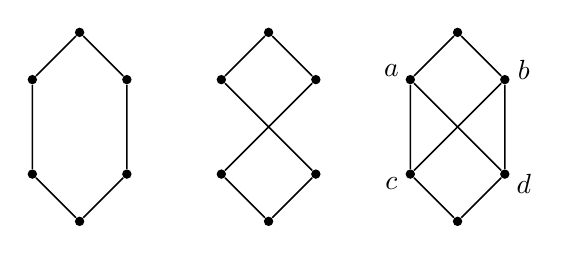
\begin{tikzpicture}[scale=0.6]
    \node (b1) at (-4,-2) [fill,circle,inner sep=1.2pt] {};
    \node (t1) at (-4,2) [fill,circle,inner sep=1.2pt] {};
    \node (b2) at (0,-2) [fill,circle,inner sep=1.2pt] {};
    \node (t2) at (0,2) [fill,circle,inner sep=1.2pt] {};
    \node (b3) at (4,-2) [fill,circle,inner sep=1.2pt] {};
    \node (t3) at (4,2) [fill,circle,inner sep=1.2pt] {};

    \node (l11) at (-5,-1) [fill,circle,inner sep=1.2pt] {};
    \node (l12) at (-3,-1) [fill,circle,inner sep=1.2pt] {};
    \node (l21) at (-1,-1) [fill,circle,inner sep=1.2pt] {};
    \node (l22) at ( 1,-1) [fill,circle,inner sep=1.2pt] {};
    \node (l31) at ( 3,-1) [fill,circle,inner sep=1.2pt] {};
    \node (l32) at ( 5,-1) [fill,circle,inner sep=1.2pt] {};

    \node (u11) at (-5,1) [fill,circle,inner sep=1.2pt] {};
    \node (u12) at (-3,1) [fill,circle,inner sep=1.2pt] {};
    \node (u21) at (-1,1) [fill,circle,inner sep=1.2pt] {};
    \node (u22) at ( 1,1) [fill,circle,inner sep=1.2pt] {};
    \node (u31) at ( 3,1) [fill,circle,inner sep=1.2pt] {};
    \node (u32) at ( 5,1) [fill,circle,inner sep=1.2pt] {};

    \draw (2.6,1.2) node {$a$};
    \draw (5.4,1.2) node {$b$};
    \draw (2.6,-1.2) node {$c$};
    \draw (5.4,-1.2) node {$d$};

    \draw[semithick] (b1) to (l11) to (u11) to (t1) to (u12) to (l12) to (b1);
    \draw[semithick] (b2) to (l21) to (u22) to (t2) to (u21) to (l22) to (b2);
    \draw[semithick] (b3) to (l31) to (u31) to (t3) to (u32) to (l32) to (b3);
    \draw[semithick] (l31) to (u32);
    \draw[semithick] (l32) to (u31);
  \end{tikzpicture}
\end{center}
\end{figure}

Note that the first two examples in Figure~\ref{fig:hasse} depict the same poset,
which illustrates that Hasse diagrams are not uniquely determined.  Also, note that the
poset represented in the first two diagrams is a lattice.  In contrast, the
poset depicted in the third diagram is not a lattice since neither $a \meet b$
nor $c \join d$ is defined -- the sets $\{a, b\}$ and $\{c, d\}$
  have upper and lower bounds, but $\{a, b\}$ has no \emph{greatest} lower
bound, and $\{c, d\}$ has no \emph{least} upper bound.

% \begin{examples}
% Figures~\ref{fig:basiclattices} and~\ref{fig:m3n5} present the
% Hasse diagrams of a few small lattices, some of which are given names the
% meaning of which will become apparent later.

%% \begin{figure}[centering]
%%   \caption{Hasse diagrams of some small lattices.}
%%   \label{fig:basiclattices}
%% \begin{center}
%% \begin{tikzpicture}[scale=0.8]

%% \draw (0,-1) node {$\mathbf{1}$};
%%   \node (0) at (0,0) [fill,circle,inner sep=1.2pt] {};

%%   \draw (2,-1) node {$\mathbf{2}$};
%%   \node (2) at (2,0) [fill,circle,inner sep=1.2pt] {};
%%   \node (21) at (2,1) [fill,circle,inner sep=1.2pt] {};
%%   \draw[semithick] (2) to (21);

%%   \draw (4,-1) node {$\mathbf{3}$};
%%   \node (3) at (4,0) [fill,circle,inner sep=1.2pt] {};
%%   \node (31) at (4,1) [fill,circle,inner sep=1.2pt] {};
%%   \node (32) at (4,2) [fill,circle,inner sep=1.2pt] {};
%%   \draw[semithick] (3) to (31) to (32);

%% \draw (6,-1) node {$\mathbf{4}$};
%%   \node (4) at (6,0) [fill,circle,inner sep=1.2pt] {};
%%   \node (41) at (6,1) [fill,circle,inner sep=1.2pt] {};
%%   \node (42) at (6,2) [fill,circle,inner sep=1.2pt] {};
%%   \node (43) at (6,3) [fill,circle,inner sep=1.2pt] {};
%%   \draw[semithick] (4) to (41) to (42) to (43);

%% \draw (9,-1) node {$\mathbf{2}\times\mathbf{2}$};
%%   \node (2x2) at (9,0) [fill,circle,inner sep=1.2pt] {};
%%   \node (2x21) at (8,1) [fill,circle,inner sep=1.2pt] {};
%%   \node (2x22) at (10,1) [fill,circle,inner sep=1.2pt] {};
%%   \node (2x23) at (9,2) [fill,circle,inner sep=1.2pt] {};
%%   \draw[semithick] (2x2) to (2x21) to (2x23) to (2x22) to (2x2);

%% \draw (12,-1) node {$\mathbf{5}$};
%%   \node (5) at (12,0) [fill,circle,inner sep=1.2pt] {};
%%   \node (51) at (12,1) [fill,circle,inner sep=1.2pt] {};
%%   \node (52) at (12,2) [fill,circle,inner sep=1.2pt] {};
%%   \node (53) at (12,3) [fill,circle,inner sep=1.2pt] {};
%%   \node (54) at (12,4) [fill,circle,inner sep=1.2pt] {};
%%   \draw[semithick] (5) to (51) to (52) to (53) to (54);

%%   \node (2x2t) at (15,0) [fill,circle,inner sep=1.2pt] {};
%%   \node (2x2t1) at (14,1) [fill,circle,inner sep=1.2pt] {};
%%   \node (2x2t2) at (16,1) [fill,circle,inner sep=1.2pt] {};
%%   \node (2x2t3) at (15,2) [fill,circle,inner sep=1.2pt] {};
%%   \node (2x2t4) at (15,3) [fill,circle,inner sep=1.2pt] {};
%%   \draw[semithick] (2x2t) to (2x2t1) to (2x2t3) to (2x2t2) to (2x2t);
%%   \draw[semithick] (2x2t3) to (2x2t4);

%%   \node (t2x2) at (18,0) [fill,circle,inner sep=1.2pt] {};
%%   \node (t2x21) at (18,1) [fill,circle,inner sep=1.2pt] {};
%%   \node (t2x22) at (17,2) [fill,circle,inner sep=1.2pt] {};
%%   \node (t2x23) at (19,2) [fill,circle,inner sep=1.2pt] {};
%%   \node (t2x24) at (18,3) [fill,circle,inner sep=1.2pt] {};
%%   \draw[semithick] (t2x2) to (t2x21) to (t2x22) to (t2x24) to (t2x23) to (t2x21);

%% \end{tikzpicture}
%% \end{center}
%% \end{figure}

%% \begin{figure}[centering]
%%   \caption{Hasse diagrams of two important lattices.}
%%   \label{fig:m3n5}
%% \begin{center}
%% \begin{tikzpicture}[scale=0.8]

%% \draw (0,-1) node {$M_3$};
%%   \node (m3) at (0,0) [fill,circle,inner sep=1.2pt] {};
%%   \node (m31) at (0,1.5) [fill,circle,inner sep=1.2pt] {};
%%   \node (m32) at (-1.5,1.5) [fill,circle,inner sep=1.2pt] {};
%%   \node (m33) at (1.5,1.5) [fill,circle,inner sep=1.2pt] {};
%%   \node (m34) at (0,3) [fill,circle,inner sep=1.2pt] {};
%%   \draw [semithick]  (m3) to (m31) to (m34) to (m33) to (m3) to (m32) to (m34);

%% \draw (6,-1) node {$N_5$};
%%   \node (n5) at (6,0) [fill,circle,inner sep=1.2pt] {};
%%   \node (n51) at (5,1) [fill,circle,inner sep=1.2pt] {};
%%   \node (n52) at (7,1.5) [fill,circle,inner sep=1.2pt] {};
%%   \node (n53) at (5,2) [fill,circle,inner sep=1.2pt] {};
%%   \node (n54) at (6,3) [fill,circle,inner sep=1.2pt] {};
%%   \draw [semithick]  (n5) to (n51) to (n53) to (n54) to (n52) to (n5);

%% \end{tikzpicture}
%% \end{center}
%% \end{figure}
%% %\end{examples}
%% \newpage










\section{Subalgebras and Homomorphisms}
Suppose $\bA = \algebra{A, F^\bA}$ is an algebra.  We call the nonempty
set $A$ the \defn{universe} of $\bA$.  \index{algebra!universe of}
If a subset $B\subseteq A$ is \emph{closed} under all
operations in $F^\bA$, we call $B$ a \defn{subuniverse} of $A$.
\index{subuniverse!defined|textit} By closed under all operations we
mean the following: for each $f\in F^\bA$, we have
$f(b_0, \dots, b_{n-1}) \in B$, for all $b_0, \dots, b_{n-1}\in B$,
where $n= \arity(f)$.

If $B\ne \emptyset$ is a subuniverse of $\algebra{A, F^\bA}$, and if we
let $F^\bB = \{f\res B : f\in F^\bA\}$, then the algebra 
$\bB = \algebra{B, F^\bB}$ is called a \defn{subalgebra} of 
$\bA$.\footnote{Here $f\res B$ denotes restriction of the
function $f$ to the set $B$ (see Appendix Sec.~\ref{sec:functions}).}  \index{subalgebra|textit}
If $\bB$ is a subalgebra of $\bA$, we denote this fact by $\bB\leq \bA$.
Similarly, we write $B\leq A$ if $B$ is a subuniverse of $A$.  We denote
the set of all subalgebras of $\bA$ by $\Sub(\bA)$.
Note that universe of an algebra is not allowed to be empty.
However, the empty set is a subuniverse.

\begin{theorem}
If $\bA_i \leq \bA$, $i\in I$, then $\bigcap A_i$ is a 
subuniverse if it is not empty.
\end{theorem}
\index{subuniverse!generated by a set|textit}
If $S$ is a nonempty subset of $A$, the \defn{subuniverse generated by} $S$, denoted
$\Sg^\bA(S)$ or $\<S\>$ is the smallest subuniverse of $\bA$ containing the set $S$.
When $\<S\> = A$, we say that $S$ generates $A$.
\begin{theorem}
If $S \subseteq A$, 
then $\Sg^\bA(S) = \< S \> = \bigcap \{ B\leq A : S\subseteq B \}$.
\end{theorem}
%% Define $\{S_i\}$ recursively as follows:
%% \begin{align*}
%% S_0 &= S;\\
%% S_{i+1} &= \{f(a_1, \dots, a_k) : \text{$f$ is a $k$-ary basic operation of $A$ and $a_i\in S_i$}\}.
%% \end{align*}
%% \begin{theorem}
%% $\Sg^\bA(S) = \< S \> = \bigcup_{i=0}^\infty S_i$.
%% \end{theorem}

Let $\bA = \< A, F^\bA \>$ and $\bB = \<B, F^\bB\>$ be algebras of the same
type, %, and let $F_n$ denote the set of $n$-ary operation symbols in $F$.
and let $\varphi : A \rightarrow B$ be a function.
Take an $n$-ary operation symbol $f\in F$, and
suppose that for %any operation symbol $f\in F_n$ and for
all $a_1, \dots a_{n}\in A$ the following equation holds:
\[
\varphi(f^\bA(a_1, \dots, a_{n})) = f^\bB(\varphi(a_1), \dots, \varphi(a_{n})).
\]
Then $\varphi$ is said to \emph{respect the interpretation of} $f$.
If $\varphi$ respects the interpretation of every $f\in F$, 
then we call $\varphi$ a \defn{homomorphism} from $\bA$ into $\bB$, and we write
$\varphi \in \Hom(\bA, \bB)$, or simply, $\varphi: \bA \rightarrow \bB$.

\medskip
\noindent {\bf Fact:} For groups, to check that a map $\varphi: G \rightarrow H$ is a
homomorphism, it is enough to check that $\varphi$ respects the interpretation
of the binary operation. It follows from this that such a function respects the
unary and nulary operations as well. (This was a homework exercise.)



\begin{example}
Let $\bG = \<G, \cdot, ^{-1}, e\>$ be a finite group of order $n$.  
Take the set $G$ (the elements of $\bG$) and consider the group of all
permutations of these elements.  We will denote this group by
$\Sym(G) = \<S, \circ, ^{-1}, \id\>$.
%% note that it is isomorphic to the symmetric group $S_n$ of permutations of
%% an $n$-element set.
Fix an element $a\in G$ and recall that the function
$\lambda_a: G \rightarrow G$, defined by $\lambda_a(g) = a\cdot g$, is a
permutation of the set $G$.  That is, $\lambda_a$ belongs to the
permutation group $\Sym(G)$.  
The function $\lambda: G \rightarrow \Sym(G)$ defined by 
$a\mapsto \lambda_a$ is a group homomorphism.\footnote{Note that the function
is given, for each $a\in G$, by $\lambda(a) = \lambda_a$.}
To see this, fix $a, b \in G$.  We must show that
the permutation 
$\lambda(a\cdot b) = \lambda_{ab}$
is the same as the permutation 
$\lambda(a) \circ \lambda(b) = \lambda_a \circ \lambda_b$.
Indeed, for all $g \in G$,
\begin{align*}
\lambda_{ab} (g) &= (a\cdot b) \cdot g = a \cdot (b \cdot g) \qquad (associativity)\\
&= a \cdot \lambda_b(g) = \lambda_a (\lambda_b(g)) \\
& = (\lambda_a \circ \lambda_b)(g).
\end{align*}
\end{example}

\section{Isomorphism Theorems}
This section covers the group theoretic versions of what are
sometimes called the \emph{Noether isomorphism theorems}.\footnote{\href{http://en.wikipedia.org/wiki/Emmy_Noether}{Emmy Noether}
(23 Mar 1882 -- 14 Apr 1935), was an influential German mathematician known
  for her groundbreaking contributions to abstract algebra and theoretical
  physics.  Ring theoretic versions of Noether's isomorphism theorems appeared
  in her 1927 paper~\cite{Noether:1927}.}
Analogs of these theorems exist for other algebraic
structures (such as rings). More generally the theorems
can be stated in a way that makes them true for all algebraic structures.  

To keep the presentation simple, we begin by stating the special
versions of the theorems that apply to groups.  However, in anticipation of 
the more general versions to come, we introduce some terminology
that will make the transition to a more general context smoother. 
For now the reader will have to trust that carrying around this slightly heavier
baggage at the start will pay off in the end. 


\subsection{The kernel: equivalence relation or subgroup?}
Let $A$ and $B$ be sets and let $\varphi : A\rightarrow B$ be a function.
We say that a pair $(a_0, a_1)\in A^2$ belongs to the \defn{kernel} of
$\varphi$, and we write $(a_0, a_1) \in \ker \varphi$, just in case
$\varphi(a_0)=\varphi(a_1)$.  Thus, to every function $\varphi :A \rightarrow B$ there corresponds a
binary relation %% $\ker \varphi$, defined 
on $A$ given by 
\[
(a_0, a_1) \in \ker \varphi \qquad \Longleftrightarrow \qquad \varphi(a_0) = \varphi(a_1).
\]

The proof of the next proposition is an easy exercise.
  \begin{prop}\label{prop:1}
    $\ker \varphi$ is an equivalence relation on the domain of $\varphi$.
  \end{prop}
\begin{exercise}  Prove proposition \ref{prop:1}. \end{exercise}
Each equivalence relation $R$ on a set $A$ partitions that set into ``blocks'' or
\emph{equivalence classes}.  
Given an element $a_1\in A$, we denote the equivalence class containing $a_1$ by
$a_1/R$, or by $[a_1]$ when the latter 
seems more convenient. Thus, a few alternative ways to write the 
equivalence class of $R$ that contains $a_1$ are as follows:
\[a_1/R = \{ a_2 \in A \mid a_1 \mathrel{R} a_2\} = \{ a_2 \in A \mid (a_1, a_2)\in R\} = [a_1].
\]
The set of all equivalence classes of a given
relation $R$ is denoted by $A/R$. That is,  
\[A/R = \bigl\{[a] : a\in A\bigr\}.\]

\begin{example}
  Suppose $A = \{w, x, y, z\}$ and $B = \{0, 1, 2\}$ and 
  let $\varphi: A \rightarrow B$ be defined by  $\varphi(w) = 2$, $\varphi(x) = 0$, and 
  $\varphi(y) = 1 = \phi(z)$. Let $R \subseteq A^2$ denote the kernel of
  $\varphi$. 
  Then, 
  \[
  R = \{(a_0, a_1) \mid \varphi(a_0) = \varphi(a_1)\} = 
  \{(w, w), (x, x), (y, y), (y, z), (z, y), (z, z)\},
  \]
  and 
  \[
  [w] = \{w\}, \qquad [x] = \{x\}, \qquad %% \text{ and } \quad 
  [y] =\{y, z\}, \qquad [z]=\{y, z\}.
  \]
  The set $A/R$ of all equivalence classes of $R$ is 
  \[
  A/R = \{[w], [x], [z]\}.
  \]
  The point is that $\varphi$ maps $y$ and $z$ to the same element, so
  the kernel ``collapses'' these points into a single class, which we can
  represent either by $[y]$ or by $[z]$.  The choice is arbitrary, since they
  both denote the same equivalence class, namely $\{y, z\}$. 
\end{example}

\begin{example}
  Suppose $\varphi: G \rightarrow H$ is a group homomorphism.  As above, the
  kernel of $\varphi$ is
  \begin{equation}
    \label{eq:1}
  \ker \varphi = \{(x, y) \in G \times G :  \varphi(x) = \varphi(y)\}
  \end{equation}
  Since $\ker \varphi$ is an equivalence relation, $G$ is partitioned into
  equivalence classes of $\ker \varphi$. 
  Let $K_\varphi$ denote the equivalence class of
  $\ker \varphi$ that contains the identity element $e_G$ of $G$.  That is,
  \[
  K_\varphi = e_G/\ker\varphi = \{x \in G :  (x, e_G) \in \ker \varphi\} =
  \{x \in G :  \varphi(x) = \varphi(e_G)\} = [e_G].
  \]
  Since $\varphi$ is a homomorphism, $\varphi(e_G) = e_H$.  Therefore,
   \[
   K_\varphi=  \{x \in G :  \varphi(x) = e_H\} =  \varphi^{-1}(\{e_H\}).
   \]
\end{example}
\begin{exercise}  Let $\varphi: G \rightarrow H$ be a group homomorphism.
  \begin{enumerate}
  \item 
    Prove that $K_\varphi$ %% = \varphi^{-1}(\{e_H\})$
    is a normal subgroup of $G$.  
  \item 
    Recall that an equivalence on $G$ partitions $G$ into disjoint equivalence
    classes.  Show that the equivalence classes of $\ker \varphi$ are precisely the
    left cosets of $K_\varphi$ in $G$; that is $\ker \varphi$ partitions $G$ into 
    the disjoint union,
    \[
    G = K_\varphi \cup g_1K_\varphi \cup g_2K_\varphi\cup \cdots.
    \]
  \end{enumerate}
\end{exercise}

\noindent  {\bf A note on terminology.} Our textbook, and most other elementary
  books on classical algebra, calls the subgroup $K_\varphi$ described above
  the ``kernel'' of $\varphi$. 
  This terminology is useful in the context of certain
  special classes of algebraic structures, such as groups or rings.  However, 
  to treat algebraic structures more generally requires
  the definition of kernel given in~(\ref{eq:1}).
  Since the two definitions of ``kernel'' serve different purposes, and since
  neither is dispensible, we must agree on a convention that will allow us to
  speak about these two notions without causing confusion. From now on, 
  \begin{itemize}
  \item ``kernel relation'' and $\ker \varphi$
    will refer to the equivalence relation defined in~(\ref{eq:1});
  \item ``kernel subgroup'' and $K_\varphi$
    will refer to the equivalence class of $\ker \varphi$ containing the
    identity.
  \end{itemize}
  We refrain from using the term ``kernel'' without qualification, unless it is
  obvious that we are referring to an equivalence relation and not a subgroup
  (or vice-versa).

  To summarize, if $\varphi: G \rightarrow H$ is a function from a set $G$ to
  a set $H$, then the 
  \defn{kernel relation} is $\ker \varphi = \{(x, y) \in G \times G :
  \varphi(x) = \varphi(y)\}$. 
  In the special case when $G$ and $H$ are groups and 
  $\varphi: G \rightarrow H$ is a group
  homomorphism, then we may speak of the \defn{kernel subgroup}, 
  $K_\varphi = \{x \in G: \varphi(x) = e_H\}$.


%%   \begin{lemma}
%%   If $\varphi: G \rightarrow H$ is a group homomorphism, then the kernel
%%   subgroup $K_\varphi$ is a normal subgroup of $G$.
%%   \end{lemma}
%%   \begin{proof}
%%     Fix $g \in G$ and $n\in N_\varphi$. Then
%%     \begin{align*}
%%     \varphi(g n g^{-1}) &= \varphi(g) \varphi(n) \varphi(g^{-1}) 
%%     \quad (\text{since $\varphi$ is a homomorphism})\\
%%     &= \varphi(g) e_H \varphi(g^{-1})
%%     \quad (\text{since $n \in N_\varphi$, so  $(n, e_G) \in \ker\varphi$})\\
%%     &= \varphi(g) \varphi(g^{-1})\\
%%     &= \varphi(gg^{-1}) \qquad (\text{since $\varphi$ is a homomorphism})\\
%%     &= \varphi(e_G)
%%     \end{align*}
%%     Therefore, $g n g^{-1}\in N_\varphi$.
%%   \end{proof}
%% \end{example}

  %% \begin{theorem}[First Isomorphism Theorem]
  %% Suppose $\varphi: G \rightarrow H$ is a group homomorphism
  %% and 
  %% \[
  %% N := \varphi^{-1}(\{e_H\}) = \{g\in G: \varphi(g) = e_H\}.
  %% \]
  %% Then there is a unique group isomorphism $\psi : G/N \rightarrow \varphi(G)$ such
  %% that $\psi \pi = \varphi$. 
  %% \end{theorem}

\subsection{Group Isomorphism Theorems}
  \begin{theorem}[First Isomorphism Theorem]
  Suppose $\varphi: G \rightarrow H$ is a group homomorphism.
  Then,
  \begin{enumerate}
  \item $K_\varphi = \varphi^{-1}(\{e_H\})$ is a normal subgroup of $G$;
  \item the image of $G$ under $\varphi$ is a subgroup of $H$;
  \item the factor group $G/K_\varphi$ is isomorphic to
    the image of $G$ under $\varphi$. 
  \end{enumerate}
  \end{theorem}
\noindent In other terms, if $\varphi: G \rightarrow H$ is a homomorphism, then
  \[
  K_\varphi \triangleleft G, \quad \varphi(G)\leq H, \quad G/K_\varphi\cong
  \varphi(G).
  \]

  %% (The conclusion says that, for all $g\in G$, 
  %% $\psi \pi(g) = \varphi(g)$ or $\psi(gN) = \varphi(g)$.)
  %% If $\varphi: G \rightarrow H$ is a group homomorphism with
  %% $N = \varphi^{-1}(\{e_H\})$, then there is a unique group homomrorphism 
  %% $\psi : G/N \rightarrow H$ such that $\psi \pi = \varphi$. 
  %% \end{theorem}
  %% The conclusion says that, for all $g\in G$, 
  %% $\psi \pi(g) = \varphi(g)$ or $\psi(gN_\varphi) = \varphi(g)$.

%%   \begin{lemma}
%% \label{lem:canonicalepi}
%%   Suppose $N$ is a normal subgroup of $G$. Then the function 
%%   $\pi: G \rightarrow G/N$ defined by $\pi(g) = gN$ is a group epimorphism with
%%   kernel subgroup $K_\pi = N$. 
%%   \end{lemma}
%%   \noindent (Recall, an \emph{epimorphism} is an onto homomorphism.)

%%   \begin{exercise}  Prove Lemma~\ref{lem:canonicalepi}.
%%   \end{exercise}

  \begin{exercise}
  Suppose $N$ is a normal subgroup of $G$. Prove that the function 
  $\pi: G \rightarrow G/N$ defined by $\pi(g) = gN$ is a group epimorphism with
  kernel subgroup $K_\pi = N$. 
  \end{exercise}

  \begin{exercise}
    Prove the First Isomorphism Theorem.
  \end{exercise}

  \begin{theorem}[Second Isomorphism Theorem]
    Let $G$ be a group with subgroups $H$ and $N$, and suppose that $N$ is a
    normal subgroup of $G$. Then 
    \begin{enumerate}
    \item $H N$ is a subgroup of $G$;
    \item $H\cap N$ is a normal subgroup of $H$;
    \item $HN/N \cong H/H\cap N$.
    \end{enumerate}
  \end{theorem}

  \begin{exercise}
    Prove the Second Isomorphism Theorem.
  \end{exercise}

  \begin{exercise}
    Let $G$ be a nonabelian simple group.  Let $S_n$ be the symmetric group of all
  permutations on an $n$-element set, and let $A_n$ be the alternating group.
    \begin{enumerate}
    \item 
      Show that if $G$ is a subgroup of $S_n$, $n$ finite, then $G$ is a subgroup
      of $A_n$.
    \item Let $H$ be a proper subgroup of $G$, and, for $g\in G$, let $\lambda_g$ be
      the map of the set of left cosets of $H$ onto themselves defined by
      $\lambda_g(xH) = gxH$.  
      Show that the map $g\mapsto \lambda_g$ is a monomorphism (injective
      homomorphism) of $G$ into the group of permutations of the set of left
      cosets of $H$. 
    \item Let $H$ be a subgroup of $G$ of finite index $n$  and assume $n>1$ (so $H \neq G$).  
      Show that $G$ can be embedded in $A_n$. (That is, show that $G$ is
      isomorphic to a subgroup of $A_n$.
    \item If $G$ is infinite, it has no proper subgroup of finite index.
    \end{enumerate}
  \end{exercise}



  \ifthenelse{\boolean{includeSolutions}}{
    \begin{solution}
      {\bf a.} Suppose $G$ is a subgroup of $S_n$, $n$ finite, and 
      assume $G$ is nonabelian and simple.  Clearly $G \neq S_n$, since $S_n$ is not simple
      (for example, $A_n \subnormal S_n$).
      Consider $G\cap A_n$. This is easily seen to be a normal subgroup of $G$.  
      (Normality: if $\sigma \in G\cap A_n$ and $g\in G$, then $g\sigma g^{-1}\in G$ and
      $g\sigma g^{-1}\in A_n$, since $A_n \subnormal S_n$, so $g\sigma g^{-1}\in G \cap
      A_n$.)  Therefore, as $G$ is simple, either $G\cap A_n = (e)$ or $G\cap A_n = G$.  
      In fact, $G\cap A_n = (e)$ never occurs under the given hypotheses, and two proofs of
      this fact are given below.  In case $G\cap A_n = G$, of course, $G\leq A_n$ and we are done.

      {\it Proof 1:} Suppose $G\cap A_n = (e)$.  Then $G$ contains only $e$ and odd
      permutations.  
      Let $\zeta\in G$ be an odd permutation.  Then $\zeta^2$ is an even permutation in $G$, so it must
      be $e$.  Thus, every nonidentity element of $G$ has order 2.  Suppose $\eta$ is
      another odd permutation in $G$. Then $\zeta \eta$ is an even permutation in $G$, so
      $\zeta \eta = e$.  Therefore, $\zeta \zeta = e = \zeta \eta$, so $\eta = \zeta$.
      This shows $G$ has only two elements $e$ and $\zeta$.  But then $G\cong \Z_2$ is abelian,
      contradicting our hypothesis. 

      {\it Proof 2:} 
      If $G$ were not a subgroup of $A_n$, then the group
      $G A_n\leq S_n$ would have order larger than $|A_n| = |S_n|/2$. 
      By Lagrange's theorem, then, it would have order
      $|S_n|$.  Therefore, $G A_n = S_n$, and, by the 
      second isomorphism theorem,
      \[
      G/(G\cap A_n) \cong G A_n/A_n = S_n/A_n.
      \]
      This rules out $G\cap A_n = (e)$, since that would give $G \cong S_n/A_n
      \cong \Z_2$ (abelian), contradicting the hypothesis.
      \qed
      ~\\
      {\bf Remark:}  Although the first proof above is completely elementary, the second is worth
      noting since it reveals useful information even when we don't assume $G$ is
      simple and nonabelian.  For example (Rose \citeRose, page 77), 
      if $G$ is a subgroup of $S_n$ containing an odd permutation, then we can show that
      exactly half of the elements of $G$ are even and half are odd.  Indeed, under these conditions
      we easily get that $G A_n = S_n$ (as in the second proof above), and then the second isomorphism
      theorem implies $|G/(G\cap A_n)| =|S_n/A_n|=2$. Therefore, $|G\cap A_n| =|G|/2$,
      which says that half the elements of $G$ belong to $A_n$, as claimed. 
      \\[12pt]
      {\bf b.} Let $H\lneq G$, and let $S$ denote the set of left cosets of $G$.  Let
      $\Sym(S)$ denote the group of permutations of $S$.  Then the map $\lambda: G\rightarrow
      \Sym(S)$ -- defined by $\lambda(g) = \lambda_g$, where $\lambda_g(xH) = gxH$ -- is a
      monomorphism of $G$ into $\Sym(S)$.  To prove this, we first show that $\lambda(g) =
      \lambda_g$ is indeed a bijection of $S$, then we show that $\lambda$ is a
      homomorphism of $G$, and finally we show that $\ker \lambda$ is $(e)$.

      To see that $\lambda_g$ is injective, observe
      \[
      \lambda_g(xH) = \lambda_g(yH) 
      \quad \Leftrightarrow \quad 
      gxH = gyH
      \quad \Leftrightarrow \quad 
      (gy)^{-1}gx \in H
      \quad \Leftrightarrow \quad 
      y^{-1}x \in H
      \quad \Leftrightarrow \quad 
      xH = yH.
      \]

      To see that $\lambda_g$ is surjective, fix $xH\in S$, and notice that
      $\lambda_g(g^{-1}xH) = gg^{-1}xH = xH$.

      To see that $\lambda$ is a homomorphism, note that, for any $xH \in S$,
      \[
      \lambda_{g_1 g_2}(xH) = g_1g_2 xH = \lambda_{g_1}(g_2 x H) = 
      \lambda_{g_1}\circ \lambda_{g_2}( x H).
      \]
      That is, $\lambda(g_1 g_2) = \lambda(g_1)\lambda(g_2)$, which proves that $\lambda$
      is a homomorphism.

      Finally, note that $\ker \lambda$ is a normal subgroup of $G$.  Therefore, as $G$ is simple,
      either $\ker \lambda = (e)$, or $\ker \lambda = G$.  But
      \[
      \ker \lambda = \{g\in G: \forall x\in G, \lambda_g(xH) = xH\} = 
      \{g\in G: \forall x\in G, x^{-1}g x \in H\} \leq H
      \]
      (since $e\in G$).  Therefore, $H\neq G$, so $\ker \lambda \neq G$, so 
      $\ker \lambda =(e)$.  This proves that $\lambda$ is a monomorphism.
      \qed
      ~\\[4pt]
      {\bf c.} Let $H$ be a subgroup of $G$ of finite index $n$ and assume $n>1$ (so $H
      \neq G$).  We must show that $G$ can be embedded into $A_n$.

      Part {\bf b.}~showed that $\lambda$ embeds $G$ into $\Sym(S)$, where $S$ is the set
      of left cosets of $H$ in $G$.  Now $[G:H] = |S| = n$, which implies
      that $\Sym(S) \cong S_n$, the group of permutations of $n$ elements.  Therefore,
      $G$ is isomorphic to a subgroup of $S_n$.  By part {\bf a.}, then, $G$ is isomorphic
      to a subgroup of $A_n$. \qed
      ~\\[4pt]
      {\bf d.} Suppose $G$ is infinite.  We must show it has no proper subgroup of finite
      index.  If, on the contrary, $H\leq G$ with $[G:H] = n$, then, $G$ would be isomorphic
      to a subgroup of the finite group $A_n$. Impossible. \qed
     \end{solution}
}




\begin{theorem}[Correspondence Theorem]\label{CorrespondTheorem}\index{Correspondence Theorem!for groups}
Let $N$ be a normal subgroup of a group $G$. Then the map
$H \mapsto H/N$
is a one-to-one correspondence between the set of subgroups of $G$ that contain 
$N$ and the set of subgroups of $G/N$. That is,
\[
\Sub(G) \; \ni \; H \; \longleftrightarrow \; H/N \; \in \; \Sub(G/N).
\]
Moreover, the
normal subgroups of $G$ containing $N$ correspond to normal subgroups of~$G/N$. 
\end{theorem}

 % Statement of the Correspondence Theorem corrected.  Suggested by P. Diethelm.  TWJ 16/8/2013.
 
 
\begin{proof}
Let $H$ be a subgroup of $G$ containing $N$. Since $N$ is normal in
$H$, $H/N$ makes sense.  Let $aN$ and $bN$ be elements of $H/N$. Then
$(aN)( b^{-1} N )= ab^{-1}N \in H/N$; hence, $H/N$ is a subgroup of
$G/N$. 


Let $S$ be a subgroup of $G/N$. This subgroup is a set of cosets of
$N$.  If  $H= \{ g \in G : gN \in S \}$, then for $h_1, h_2 \in H$, we
have that $(h_1 N)( h_2 N )= h_1 h_2 N \in S$ and $h_1^{-1} N \in S$.
Therefore, $H$ must be a subgroup of $G$. Clearly, $H$ contains $N$.
Therefore, $S = H / N$. Consequently, the map  $H \mapsto H/N$ is
onto. 

% Notation error corrected.  Suggested by P. Diethelm.  TWJ 16/8/2013.
    
Suppose that $H_1$ and $H_2$ are subgroups of $G$ containing $N$ such
that $H_1/N = H_2/N$. If $h_1 \in H_1$, then $h_1 N \in H_1/N$. Hence,
$h_1 N = h_2 N \subset H_2$ for some $h_2$ in $H_2$. However, since
$N$ is contained in $H_2$, we know that $h_1 \in H_2$ or $H_1 \subset
H_2$. Similarly, $H_2 \subset H_1$.  Since $H_1 = H_2$, the map  $H
\mapsto H/N$ is one-to-one. 

%H/N changed to N/H.  Suggested by S. Engle.
%TWJ - 12/19/2011

%Changed it back.  What was I thinking?  Suggested by R. Beezer.
%TWJ - 11/29/2012


 
Suppose that $H$ is normal in $G$ and $N$ is a subgroup of $H$.  Then
it is easy to verify that the map $G/N \rightarrow G/H$ defined by $gN
\mapsto gH$ is  a homomorphism.  The kernel of this homomorphism is
$H/N$, which proves that $H/N$ is normal in $G/N$. 
 
 
Conversely, suppose that $H/N$ is normal in $G/N$. The homomorphism
given by 
\[
G \rightarrow G/N \rightarrow \frac{G/N}{H/N}
\]
has kernel $H$. Hence, $H$ must be normal in $G$.
\end{proof}
 
\medskip
 
 
Notice that in the course of the proof of Theorem~\ref{CorrespondTheorem}, we have also
proved the following theorem. 
 



  \begin{theorem}[Third Isomorphism Theorem]
    Let $N \leq H \leq G$ be a chain of groups and suppose $N$ and $H$ are both
    normal in $G$. Then,
    \[
    G/H \cong \frac{G/N}{H/N}.
    \]
  \end{theorem}
 
 
  \begin{example}
    Fix two integers $m, n \in \Z$.  By the Third Isomorphism Theorem,
    \[
      {\mathbb Z} / m {\mathbb Z} \cong ({\mathbb Z}/ mn {\mathbb Z})/ (m {\mathbb Z}/ mn
      {\mathbb Z}). 
      \]
      Since $| {\mathbb Z} / mn {\mathbb Z} | = mn$ and  
      $|{\mathbb Z} / m{\mathbb Z}| = m$, 
      we have $| m {\mathbb Z} / mn {\mathbb Z}| = n$. 
  \end{example}
 


\section{Quotient Algebras}
\index{quotient algebra}
Let $\bA = \<A, F\>$ be an algebra.  Recall, $F$ denotes the set of operation symbols,
and to each operation symbol $f\in F$ there corresponds an arity, and the set of
arities determines the similarity type of the algebra.  (We might do better to
denote the algebra by $\<A, F^\bA\>$, since the algebra is not defined 
until we have associated to each operation symbol $f\in F$ an actual operation
$f^\bA$ on $A$, but this is a technical point, and we will often denote two
algebras of the same similarity type as $\<A, F\>$ and $\<B, F\>$ with the
understanding that the meaning of $F$ depends on the context.)

Let $\theta \in \Con\bA$ be a congruence relation.  The \defn{quotient algebra}
$\bA/\theta$ is an algebra with the same similarity type as $\bA$, with universe
$A/\theta = \{a/\theta : a\in A\}$, and operation symbols $F$, where for each
($k$-ary) symbol $f\in F$  the operation $f^{\bA/\theta}$ is defined as follows:
for $(a_1/\theta, \dots, a_k/\theta) \in (A/\theta)^k$, 
\[
f^{\bA/\theta}(a_1/\theta, \dots, a_k/\theta) = 
f^{\bA}(a_1,\dots, a_k)/\theta. % \; \in \; A/\theta.
\]
(As mentioned above, $F$ denotes the set of operation symbols of the
similarity type of the algebra, and it is ``overloaded''  in the sense that we
write $\bA = \<A, F\>$ and $\bA/\theta = \<A/\theta, F\>$, and for each
$f\in F$ the corresponding operation in these algebras is interpreted
appropriately---i.e., as $f^\bA$ or $f^{\bA/\theta}$.) 

\section{Direct Products of Algebras}
\label{sec:directproducts}
\index{direct product!of algebras}
Above we defined direct products of sets.  We now define direct products of
algebras.  Let $\bA = \<A, F\>$ and $\bB = \<B, F\>$ be two algebras of the same
similarity type.  The \defn{direct product} $\bA \times \bB$ is an
algebra of the same type as $\bA$ and $\bB$, with universe $A \times
B = \{(a, b) : a\in A, b\in B\}$, and operation symbols $F$.  To each ($k$-ary)
symbol $f\in F$ corresponds an operation $f^{\bA \times \bB}$ defined as follows:
for $((a_1, b_1), \dots, (a_k, b_k)) \in 
(A\times B)^k$,
\begin{equation}
  \label{eq:prod}
f^{\bA\times \bB}
((a_1, b_1), \dots, (a_k, b_k)) =
(f^{\bA}(a_1, \dots, a_k),f^{\bB}(b_1, \dots, b_k)).
\end{equation}
This definition can be easily extended to the direct product $\prod \bA_i$ of
any collection of algebras $\{\bA_i : i\in I\}$, and we leave it to the reader
to write down the defining property of the operations, which is completely
analogous to (\ref{eq:prod}).  

\index{direct power|textit}
If all the algebras are isomorphic %% ---that is,
%% when $\bA_i= \bA$, for some $\bA$---
we sometimes call 
$\prod \bA_i$ the \defn{direct power} of $\bA$.  When the set $I$ is
finite, say, $I = {1, 2, \dots, n}$,
%$\{\bA_i : i\in I\} = \{\bA_1, \bA_2, \dots, \bA_n\}$,
we have alternative notations for the direct power, namely,
\[
\prod \bA_i = \bA_1 \times \bA_2 \times \cdots \times \bA_n = \bA^n.
\]

The constructions of this section and the preceding one
are often combined to give direct products of quotient algebras.  For instance, if
$\theta_1$ and $\theta_2$ are two congruences of $\bA$, the algebra 
$\bA/\theta_1\times \bA/\theta_2$ has the same similarity type as $\bA$, and its
universe is
\[
A/\theta_1\times A/\theta_2 = \{
(a/\theta_1, b/\theta_2) : a, b \in A\}.
\]
The operation symbols are again $F$, and to each ($k$-ary) symbol $f\in F$
corresponds an operation $f^{\bA/\theta_1\times \bA/\theta_2}$ defined as follows:
 for $((a_1/\theta_1, b_1/\theta_2), \dots, (a_k/\theta_1, b_k/\theta_2)) \in 
(A/\theta_1\times A/\theta_2)^k$,
 \begin{align*}
f^{\bA/\theta_1\times \bA/\theta_2}
((a_1/\theta_1, b_1/\theta_2), \dots, (a_k/\theta_1, b_k/\theta_2))
&=
(f^{\bA/\theta_1}
(a_1/\theta_1, \dots, a_k/\theta_1),
f^{\bA/\theta_2}
(b_1/\theta_2, \dots, b_k/\theta_2))\\
&=
(f^{\bA}(a_1, \dots, a_k)/\theta_1,
 f^{\bA}(b_1, \dots, b_k)/\theta_2). %\; \in \; A/\theta_1 \times A/\theta_2.
 \end{align*}


\appendix                       

\begin{center}
  APPENDIX
\end{center}


\section{Examples of Algebraic Structures}
\label{sec:exampl-algebr-struct}
Recall from above that an \emph{algebra}
$\bA$ is an ordered pair $\bA = \langle A, F\rangle$ 
where $A$ is a nonempty set and $F$ is a family of finitary operations on $A$.
The set $A$ is called the universe of \bA, and the elements $f^{\bA} \in F$ are 
called the fundamental operations of $\bA$. (In practice we prefer to 
write $f$ for $f^{\bA}$ when this doesn't cause
ambiguity.The \emph{arity} of an operation is the number of operands upon which it
acts, and we say that $f\in F$ is an $n$-\emph{ary} operation on
$A$ if $f$ maps $A^n$ into $A$.
An operation $f\in F$ is called a \emph{nullary} operation (or constant) 
if its arity is zero.  \emph{Unary}, \emph{binary}, and \emph{ternary} 
operations have arity 1, 2, and 3, respectively.  An algebra \bA\ is called 
\emph{unary} if all of its operations are unary.  An algebra \bA\ 
is \emph{finite} if $|A|$ is finite and \emph{trivial} if $|A| = 1$.
Given two algebras $\bA$ and $\bB$, we say that $\bB$ is a 
\emph{reduct} of $\bA$ if both algebras have the same universe and $\bA$
is obtained from $\bB$ by simply adding more operations.

Below is a list of a few of the most basic algebraic structures. 
A list of \emph{many} more can be found at
{\small \url{http://www.math.chapman.edu/~jipsen/structures/doku.php/index.html}}.

\begin{itemize}
\item[\emph{magma}] $\bA = \langle A, \cdot\rangle$ \\
An algebra with a single binary operation is called a \emph{magma} 
(or groupoid or binar). This operation is 
usually denoted by $+$ or $\cdot$, and we write $a+b$ or $a\cdot b$ 
(or just $ab$) for the image of $(a, b)$ under
this operation, and call it the sum or product of $a$ and $b$, respectively.

\item[\emph{semigroup}] $\bA = \langle A, \cdot\rangle$ \\
A groupoid for which 
the binary operation is associative is called a \emph{semigroup}. That is,
a semigroup is a groupoid with binary operation satisfying 
$(a\cdot b)\cdot c = a\cdot (b\cdot c)$, for all $a, b, c \in A$.

\item[\emph{monoid}] $\bA = \langle A, \cdot, e\rangle$\\
 A \emph{monoid} 
  is a semigroup along with a \emph{multiplicative identity} $e$. That is, 
$\langle A, \cdot \rangle$ is a semigroup and $e$ is a constant 
(nullary operation) satisfying $e\cdot a = a\cdot e = a$, for all $a\in A$.

\item[\emph{group}] $\bA = \langle A, \cdot, ^{-1}, e\rangle$\\
A \emph{group} is a monoid along with a unary operation $^{-1}$ called \emph{multiplicative inverse}.
That is, the reduct $\langle A, \cdot, e \rangle$ is a monoid and
$^{-1}$ satisfies $a\cdot a^{-1} =  a^{-1}\cdot a = e$, for all $a\in A$. 
An \emph{Abelian group} is a group with a commutative binary
operation, which we usually denote by $+$ instead
of $\cdot$.  In this case, we write $0$ instead of $e$ to
denote the \emph{additive identity}, and $-$ instead of
$^{-1}$ to denote the \emph{additive inverse}.  Thus, an Abelian
group is a group $\bA = \langle A, +, -, 0\rangle$ such that 
$a+b = b+a$ for all $a, b \in A$.

%% \item[\emph{ring}] $\bA = \langle A, +, \cdot,  -, 0\rangle$\\
%% A \emph{ring} is an algebra $\bA = \langle A, +, \cdot, -, 0\rangle$ such that 
%% \begin{enumerate}
%% \item[R1.] $\langle A, +, -, 0\rangle$ is an Abelian group, 
%% \item[R2.] $\langle A, \cdot \rangle$ is a semigroup, and 
%% \item[R3.] for all $a, b, c \in A$, $a\cdot(b+c)= a\cdot b + a\cdot c$ and $(a+b)\cdot c = a\cdot c + b\cdot c$.
%% \end{enumerate}

%% A \emph{ring with unity} (or \emph{unital ring}) is an algebra 
%% $\bA = \langle A, +,\cdot,  -, 0, 1\rangle$, where the reduct 
%% $\langle A, +, \cdot, -,0\rangle$ is a ring, and where $1$ is a multiplicative 
%% identity; i.e.~$a\cdot 1 = 1\cdot a = a$, for all $a\in A$.

%% %% \item[\emph{field}] If $\bA = \langle A, +, \cdot, -, 0, 1\rangle$ is a ring with
%% %%   unity, an element $r\in A$ is called a \emph{unit} if it has a multiplicative
%% %%   inverse. That is, $r\in A$ is a unit provided there exists $r^{-1} \in A$ with
%% %%   $r\cdot r^{-1}  = r^{-1} \cdot  r = 1$. 
%% %%   A \emph{division ring} is a ring in which every non-zero element is a unit, and 
%% %%   a \emph{field} is a division ring in which multiplication is commutative.

\end{itemize}

%% %\newpage
%% \subsection{Vector Spaces, Modules, and Bilinear Algebras}
%% \begin{itemize}
%% \item[\emph{module}] Let $\bR = \langle R, +, \cdot, -, 0, 1\rangle $ be a ring with
%%   unit.  An  $R$-\emph{module} (sometimes called a \emph{left unitary $R$-module}) is an
%% algebra $\bM = \langle M, +, -, 0, f_r\rangle_{r\in R}$ with an Abelian group reduct
%% $\langle M, +, -, 0\rangle$, and with unary operations $(f_r)_{r\in R}$ which
%% satisfy the following four conditions for all $r, s\in R$ and $x, y \in M$:
%% \begin{enumerate}
%% \item[M1.] $f_r(x + y)  = f_r(x) + f_r(y)$
%% \item[M2.] $f_{r+s}(x) = f_r(x) + f_s(x)$
%% \item[M3.] $f_r(f_s(x)) = f_{rs}(x)$
%% \item[M4.] $f_1(x) = x$.
%% \end{enumerate}
%% If the ring $R$ happens to be a field, an $R$-module is typically called a \emph{vector space
%%   over} $R$.  

%% Note that condition M1 says that each $f_r$ is an endomorphism of the
%% Abelian group $\langle M, +, -, 0\rangle$.  Conditions M2--M4 say: (1) the
%% collection of endomorphisms $(f_r)_{r\in R}$ is itself a ring with unit, where
%% the function composition described in (M3) is the binary multiplication operation,
%% and (2) the map $r\mapsto f_r$ is a ring epimorphism from $\bR$ onto $(f_r)_{r\in R}$.

%% Part of the importance of modules lies in the fact that every ring is, up to
%% isomorphism, a ring of endomorphisms of some Abelian group.  This fact is analogous
%% to the more familiar theorem of Cayley stating that every group is isomorphic to a
%% group of permutations of some set.

%% \item[\emph{bilinear algebra}] Let $\bF = \langle F, +, \cdot, -, 0, 1\rangle$ be a
%%   field.  An algebra $\bA = \langle A, +, \cdot, -, 0, f_r\rangle_{r\in F}$ is a
%%   \emph{bilinear algebra over} $\bF$ provided 
%%   $\langle A, +, \cdot, -, 0, f_r\rangle_{r\in F}$ is a vector space over $\bF$ and
%%   for all $a, b, c \in A$ and all $r\in F$, 
%%     \begin{align*}
%%       (a + b)\cdot c &= (a\cdot c) + (b\cdot c)\\
%%       c \cdot (a + b)&= (c\cdot a) + (c\cdot b)\\
%%       a\cdot f_r(b) &= f_r(a\cdot b) = f_r(a)\cdot b
%%     \end{align*}
%% If, in addition, $(a \cdot b)\cdot c = a\cdot (b\cdot c)$ for all $a, b, c \in A$,
%% then $\bA$ is called an \emph{associative algebra over} $\bF$.  Thus an associative
%% algebra over a field has both a vector space reduct and a ring reduct.  An example of
%% an associative algebra is the space of linear transformations (endomorphisms) of any
%% vector space into itself.
%% \end{itemize}



\section{Prerequisites}
This section gives a brief review of some elementary definitions and facts
from set theory.
See Enderton~\cite{Enderton:1977} for more details.
\subsection{Tuples and Relations}
\label{sec:relations}
Most of us probably have a good idea of what is meant by an
``ordered pair,'' $(x, y)$.  It consists of two elements (or sets) 
$x$ and $y$, listed in a particular order.  
How to make this notion mathematically precise is not quite
so obvious.  According to~\cite{Enderton:1977}, in 1921 Kazimierz
Kuratowski gave us the definition in general use today: given two
sets $x$ and $y$, the \defn{ordered pair} $(x, y)$ is defined to be the set
$\{\{x\}, \{x, y\}\}$. 
It is not too hard to prove that this definition captures our
intuitive idea of ordered pair---namely, $(x, y)$ uniquely determines both
what $x$ and $y$ are, and the order in which they appear.  Indeed, it is a
theorem (Theorem 3A of~\cite{Enderton:1977}) that $(u, v) = (x, y)$ iff $u =
x$ and $v = y$. 

A \defn{binary relation} is a set of ordered pairs.  Thus, if $X$ is a set, a
binary relation $R$ on $X$ is simply a subset of the Cartesian product, that is,
\[
R \subseteq X\times X := \{(x_1, x_2) : x_1, x_2 \in X\}.
\]
For a binary relation $R$, we sometimes write $x \rR y$ in place of $(x, y) \in R$. 
For example, in the case of the order relation $\leq$ on the set \R\ of real numbers,
$\leq$ is defined to be the set 
\[
\{(x, y) \in \R \times \R : \text{$x$ is less than or equal to $y$}\},
\]  
and we usually write $x \leq y$ to mean that the pair 
$(x, y)$ belongs to the relation $\leq$.  Of course, we could write
$(x, y) \in \; \leq$, but the ``infix'' notation $x \leq y$ is often
preferred for binary relations. 


For a relation $R$, we define the \defn{domain} of $R$ ($\dom R$) and the 
\defn{range} of $R$ ($\ran R$) %% , and the \defn{field} of $R$ ($\fld R$)
by
\begin{align*}
x \in  \dom R \quad &\Longleftrightarrow \quad \exists y \; (x,y) \in R,\\
x \in\ran R  \quad &\Longleftrightarrow \quad \exists t \; (t,x) \in R.%% ,\\
%% \fld R &= \dom R \cup \ran R.
\end{align*}

%% \item {\bf $n$-ary relations.}
We can extend the definition of ordered pairs and define an 
\emph{ordered triple} recursively, as follows:
\[
(x, y, z) = ((x, y), z).
\]
Similarly we can form \emph{ordered quadruples}:
\[
(x_1, x_2, x_3, x_4) = ((x_1, x_2, x_3), x_4)
= (((x_1,x_2),x_3),x_4).
\]
Inductively, for each $n\in \N$, if we assume the notion of ordered $k$-tuple,
$(x_1, \dots, x_k)$, has been defined for $k < n$, we can form 
\emph{ordered $n$-tuples} as follows:
\[
(x_1, \dots, x_{n-1}, x_n) = ((x_1, \dots, x_{n-1}), x_n).
\]
%% Clearly we could continue in this way to define ordered quintuples or ordered
%% $n$-tuples for any particular $n$. 
It is convenient for reasons of uniformity to
define also the 1-tuple $(x) = x$.
We define an $n$-ary relation on $A$ to be a set of ordered $n$-tuples with all
components in $A$. Thus a binary (2-ary) relation on $A$ is just a subset of
$A \times A$. And a ternary (3-ary) relation on $A$ is a subset of 
$(A \times A) \times A$.
There is, however, a terminological quirk here. If $n > 1$, then any $n$-ary
relation on $A$ is actually a binary relation, but a unary (1-ary) relation on $A$ is just
a subset of $A$. %% ; thus it may not be a binary relation at all.

A relation $R$ on a set $A$ is called \defn{reflexive} iff $x \rR x$ for all 
$x \in A$; \defn{symmetric} iff whenever $x\rR y$ then also
$y\rR x$; \defn{transitive} iff whenever $x\rR y$ and $y\rR z$,
then also $x\rR z$.  A relation is an \defn{equivalence relation} 
iff it is a binary relation that is reflexive, symmetric, and transitive.  Given
a set $A$, we denote the set of all equivalence relations on $A$ by $\Eq(A)$.

\subsection{Functions}
\label{sec:functions}
A \defn{function} (or mapping) is a relation $F$ such that for each $x$ in $\dom F$ there
is only one $y$ such that $x \,F\, y$.

The following operations are most commonly applied to functions, are
sometimes applied to relations, but can actually be defined for arbitrary
sets $A$, $F$, and $G$.

\begin{enumerate}[(a)]
\setlength{\itemsep}{0.0ex plus0.1ex}
\item The \defn{inverse} of $F$ is the set
\[
F^{-1}=\{(u, v) \mid v \,F \,u\}=\{(u, v) \mid (v,u) \in F \}.
\]
\item  The \defn{composition} of $F$ and $G$ is the set
\[
F \circ G = \{(u, v) \mid \exists t \,(u \,G \,t \;\&\; t\, F\, v)\}
= \{(u, v) \mid \exists t \;((u,t)\in G\; \& \;(t,v) \in F)\}.
\]
\item The \defn{restriction} of $F$ to $A$ is the set
\[
F \res A = \{(u, v) \mid u \, F \,v\; \& \; u \in A\}
= \{(u, v) \mid (u,v)\in F \; \& \; u \in A\}.
\]
\item  The \defn{image} of $A$ under $F$ is the set
\[
F\lb A\rb = \ran(F \res A)= \{v \mid (\exists u \in A)\; (u,v) \in F\}.
\]
\end{enumerate}
$F\lb A\rb$ can be characterized more simply when $F$ is a function and
$A\subseteq \dom F$; in this case
\[
F\lb A\rb = \{F(u) \mid u \in A\}.
\]
In each case we can easily apply a subset axiom to establish the
existence of the desired set. Specifically, 
\[
F^{-1} \subseteq \ran F \times \dom F, \quad 
F \circ G \subseteq \dom G \times \ran F, \quad  
F \res A \subseteq F, \quad 
F\lb A\rb \subseteq \ran F.
\]
(A more detailed justification of the definition of 
$F^{-1}$ would go as follows: By a subset axiom
there is a set $B$ such that for any $x$,
\[
x\in B \quad \Longleftrightarrow \quad  x \in  \ran F \times \dom F \; \& \; 
\exists u \; \exists v\; (x = (u, v) \; \&\; (v, u) \in F).
\]
It then follows that
\[
x\in B \quad \Longleftrightarrow  \quad \exists u \; \exists v\; (x = (u, v) \; \&\; (v, u) \in F).
\]
This unique set $B$ we denote by $F^{-1}$.)\\[8pt]
\begin{example}
Let
\[
F = \{ (\emptyset, a), (\{\emptyset\}, b) \}.
\]
Observe that $F$ is a function. We have $F^{-1} = \{ (a, \emptyset), (b, \{\emptyset\}) \}$.
Thus, $F^{-1}$ is a function iff $a \neq b$. The restriction of $F$ to $\emptyset$ is $\emptyset$, but
$F \res \{\emptyset\} = \{(0, a)\}$.
Consequently, $F\lb \{\emptyset \}\rb = \{a\}$, in contrast to the fact that $F(\{\es\}) = b$.
\end{example}

\begin{theorem}
Assume that $F: A\rightarrow  B$, and that $A$ is nonempty.
  \begin{enumerate}[(a)]
\setlength{\itemsep}{0.0ex plus0.1ex}
  \item There exists a function $G: B \rightarrow A$ (a ``left inverse'') such that $G \circ F$
    is the identity function $\id_{A}$ on $A$ iff $F$ is one-to-one.
  \item There exists a function $H: B \rightarrow A$ (a ``right inverse'') such that $F \circ H$
    is the identity function $\id_{B}$ on $B$ iff $F$ maps $A$ \emph{onto} $B$.
  \end{enumerate}
\end{theorem}

\noindent 
{\bf Axiom of Choice 1.} For any relation $R$ there is a function
$H \subseteq R$ with $\dom H = \dom R$.

With this axiom we can prove the sufficiency direction of part (b) of the Theorem above:
take $H$ to be a function with $H \subseteq F^{-1}$ and $\dom H = \dom F^{-1} = B$. Then
$H$ does what we want: Given any $y \in B$, we have $(y,H(y)) \in F^{-1}$ hence
$(H(y), y) \in F$, and so $F(H(y)) = y$.
\qed

\bibliographystyle{plain}
\bibliography{wjd}
\printindex

\end{document}





\section{Notation}
\begin{itemize}
\item $A^A$, the set of maps from a set $A$ into itself.
\item $\Aut(\bA)$, the group of automorphisms of an algebra $\bA$.
\item $\End(\bA)$, the set of endomorphisms an algebra $\bA$.
\item $\Hom(\bA, \bB)$, the set of homomorphism from an algebra $\bA$ into an algebra $\bB$.
\item $\Con(\bA)$, the set of congruence relations of an algebra $\bA$.
\item $\bCon \bA$, the lattice of congruence relations of an algebra $\bA$.
\item $\Eq(A)$, the set of equivalence relations of a set $A$.
\item $\bEq \bA$, the lattice of equivalence relations of a set $A$.
\item $\Sub(\bA)$, the set of subalgebras of an algebra $\bA$.
\item $\bSub \bA$, the lattice of subalgebras of an algebra $\bA$.
\item $\Sg^\bA(X)$, the subuniverse of $\bA$ generated by a set $X\subseteq A$.
\item $\N = \{1, 2, \dots\}$, the set of natural numbers.
\item $\Z = \{\dots, -1, 0, 1, \dots\}$, the set of integers.
\item $\R = (-\infty, \infty)$, the set of real numbers.
\item $\C$, the set of complex numbers.
\item $\Q$, the set of rational numbers.
\end{itemize}



















\subsection{Congruence Relations}

Let $\bA = \< A, F^\bA \>$ and $\bB = \<B, F^\bB\>$ be algebras of the same type
and let $\varphi : A \rightarrow B$ be a homomorphism.  As above, 
$\varphi$ determines an equivalence relation $\sim_\varphi = \ker \varphi$ on $A$.
\index{congruence relation|textit}
Such equivalence relations are called \emph{congruence relations}.
That is, a \defn{congruence relation} on $\bA$ is the kernel of 
a %% an equivalence relation $\sim_\varphi$
%% arising from a 
\emph{homomorphism} $\varphi : \bA \rightarrow \bB$, for some algebra
$\bB$.  We denote the set of all congruence relations on $\bA$ by $\Con \bA$.

To reiterate, $\theta \in \Con \bA$ if and only if $\theta = \ker \varphi$ for some 
homomorphism $\varphi$ of $\bA$.  There is an alternative but equivalent way to
define congruence relation of an algebra---namely, \emph{a congruence relation
is an equivalence relation that is respected by all operations of the algebra.}
That is, $\theta \in \Eq(A)$ and for every operation $f\in F$ 
(say, $n$-ary) we have
\begin{equation}
\label{eq:cong-re}
(x_i, y_i) \in \theta \; (1\leq i \leq n) \quad \Longrightarrow \quad 
(f(x_1, \dots, x_{n}), f(y_1, \dots, y_{n})) \in \theta,
\end{equation}
for all $x_1, \dots, x_{n}, y_1, \dots, y_{n} \in A$.\footnote{Another way to
  say this is $\Con \bA = \Eq(A) \cap \Sub(\bA\times \bA)$.
The direct product algebra $\bA \times \bA$ is defined in section~\ref{sec:directproducts}.}
We record this fact as
\begin{theorem}
  \label{thm:cong-rel}
  Suppose $\bA = \algebra{A, F}$ is an algebra and $\theta$ is an equivalence
  relation on the set $A$.  Then $\theta$ is congruence relation on the algebra
  $\bA$ if and only if %(for every $n$ in the similarity type of $\bA$) 
  for every $n$-ary basic operation $f\in F$  and for all
  $a_0, \dots, a_{n-1}, a_0', \dots, a_{n-1}' \in A$,
  \[
  x_i \rel{\theta} y_i \; (1\leq i \leq n) \quad \Longrightarrow \quad 
  f(x_1, \dots, x_{n}) \rel{\theta} f(y_1, \dots, y_{n}).
  \]
\end{theorem}
  In fact, we can replace the final implication in the theorem with: for each $1
  \leq i \leq n$,
  \[
  x_i\rel{\theta} y_i   \quad \Longrightarrow \quad 
  f(x_1, \dots, x_i, \dots x_{n})\rel{\theta} f(y_1, \dots,
  y_i, \dots, y_{n}).
  \]
  \underline{Proof sketch:} Recall that $a/\theta$ denotes the equivalence class of
  $\theta$ which contains $a$, and $A/\theta$ denotes the full set of $\theta$
  classes: $A/\theta= \{a/\theta : a\in A\}$.  For every
  operation $f^\bA$ on $A$ (say $n$-ary), \emph{define} an operation on
  $A/\theta$ as follows:
  \[
  f^{\bA/\theta}(a_1/\theta, \dots, a_n/\theta) := f^\bA(a_1, \dots, a_n)/\theta. 
  \]
  One easily checks that this is well-defined and that the map 
  $a \mapsto a/\theta$ is a homomorphism of $\bA$ onto the algebra 
  $\bA/\theta := \<A/\theta, F^{\bA/\theta}\>$, where 
  $F^{\bA/\theta} := \{f^{\bA/\theta} : f^\bA \in F\}$.  Finally, note that the
  kernel of this homomorphism is $\theta$.









Let \bA\ and \bB\ be algebras of the same type and let
$f : \bA \rightarrow \bB$ be a homomorphism.  Suppose 
$g$ is another homomorphism on \bA.
\begin{figure}[h]
  \caption{The Isomorphism Theorem}
  \label{fig:secondhom}
  \begin{center}
    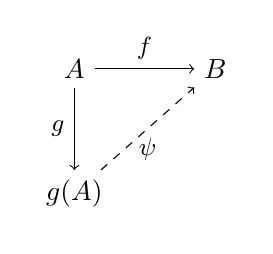
\begin{tikzpicture}
      \matrix (m) [matrix of math nodes, row sep=3em,column sep=3em]
      { A & B \\
        g(A)&\\ };
      \path[->,font=\small]
      (m-1-1) edge node[above] {$f$} (m-1-2)
      edge node[left] {$g$} (m-2-1);
      \path[->, dashed,font=\small]
      (m-2-1) edge node[below] {$ \psi $} (m-1-2);
    \end{tikzpicture}
  \end{center}
\end{figure}
Take a look at Figure~\ref{fig:secondhom} and ask yourself
what hypothesis would ensure the existence of a
function $\psi : g(A) \rightarrow B$ such that the composition $\psi \circ g$ is
equivalent to the function $f$ (in which case we say that the diagram ``commutes''). 

The first thing to note is that we must have
$\ker g \subseteq \ker f$, since $(x,y)\in \ker g$ if and only if
$g(x) = g(y)$ only if $\psi g(x) = \psi g(y)$.  

Now $g$ is a homomorphism, so $g(A)$ is a subuniverse of some
algebra, and we will see that $\ker g \subseteq \ker f$ is, in fact, 
the only hypothesis we need to ensure that there exists a \emph{homomorphism}
$\psi$ from the subalgebra $\mathbf{g(A)}$ (abusing notation) into the algebra $\bB$
with $\psi g = f$.

\begin{figure}[h,centering]
  \caption{Proof of the 2nd Isomorphism Theorem}
  \label{fig:secondhomproof}
  \begin{center}
    \begin{tikzpicture}
      \draw[dashed,blue] (-.15,0.1) rectangle (4.15,1.1);
      \draw[dashed,red] (-.15,1.2) rectangle (4.15,2.1);
      \draw[dashed,green] (-.15,2.2) rectangle (4.15,3.1);
      \draw[dashed] (-.15,3.2) rectangle (4.15,4.1);

      \draw (0,0.2) rectangle (1.5,1)
      (1.6,0.2) rectangle (2,1)
      (2.1,0.2) rectangle (3,1)
      (3.1,0.2) rectangle (3.3,1)
      (3.4,0.2) rectangle (3.6,1)
      (3.7,0.2) rectangle (4,1);
      \fill (.3,.4) circle (1pt);
      \draw (.55,.4) node {$a_0$};
      \fill (1,.6) circle (1pt);
      \draw (1.25,.6) node {$a_1$};
      \fill (2.3,.4) circle (1pt);
      \draw (2.55,.4) node {$a_2$};

      \draw (0,1.3) rectangle (2,2)
      (2.1,1.3) rectangle (3,2)
      (3.1,1.3) rectangle (4,2);
      \fill (1.4,1.6) circle (1pt);
      \draw (1.65,1.6) node {$a_3$};

      \draw (0,2.3) rectangle (2.5,3)
      (2.6,2.3) rectangle (4,3);

      \draw (0,3.3) rectangle (1.2,4)
      (1.3,3.3) rectangle (2.3,4)
      (2.4,3.3) rectangle (2.6,4)
      (2.7,3.3) rectangle (4,4);
      % \fill (3.3,3.4) circle (1pt);
      % \draw (3.55,3.4) node {$a_4$};

      \path[->,font=\scriptsize]
      (4.3,.5) edge (6.5,.5);
      \path[->,font=\scriptsize]
      (4.3,1.5) edge  (6.25,1.5);
      \path[->,font=\scriptsize]
      (4.3,2.5) edge  (6.5,2.5);
      \path[->,font=\scriptsize]
      (4.3,3.5) edge (6.5,3.5);

      \draw[dotted] (6.7,2) ellipse (.7cm and 2.2cm);
      \draw (6.95,3.5) node {$b_3$};
      \fill (6.7,3.5) circle (2pt);
      \draw (6.95,2.5) node {$b_2$};
      \fill[green] (6.7,2.5) circle (2pt);
      \draw (6.65,1.5) node {$b_1$};
      \fill[red] (6.4,1.5) circle (2pt);
      \draw (6.95,.5) node {$b_0$};
      \fill[blue] (6.7,.5) circle (2pt);

      \draw(9,1.5) node {$b_1=f(a_3)$};
      \draw(10,.5) node {$b_0=f(a_0)=f(a_1)=f(a_2)$};

      \draw[font=\LARGE] (-1,3) node {$A$};
      \draw[font=\LARGE] (7.8,3) node {$B$};
      \draw[font=\LARGE] (-.5,-3) node {$g(A)$};
      \draw[font=\large] (5.25,4) node {$f$};
      \draw[blue] (-1.2,.5) node {$a_0/ker f$};
      \draw[blue] (-.5,.5) -- (-.3,.5);
      \draw (.4,-.5) node {$a_0/ker g$};
      \draw (.7,-.2) -- (.9,.3);

      \draw[font=\large] (1.7,-.9) node {$g$};
      % \draw[->,thick] (.3,-.2) to [out=230,in=100] (0,-1.5);
      \path[->,font=\scriptsize] (2,-.2) edge (2,-1.8);

      \draw[font=\large] (6.5,-3) node {$\psi$};
      \draw[->,loosely dashed, red] (4.2,-4) to [out=30,in=-100] (6.35,1.2);
      \draw[->,loosely dashed, blue] (4.2,-4.9) to [out=30,in=-100] (6.7,.2);


      % \draw(-1.5,-5.8) node {$g(a_0)=g(a_1)$};
      % \draw[->,semithick] (-.4,-5.7) to [out=15,in=225] (.5,-5.3);
      % \draw[dotted] (2,-3.7) ellipse (3.5cm and 2.3cm);

      \draw(-1.1,-5.5) node {$g(a_0)=g(a_1)$};
      \draw (0,-5.4) -- (.8,-5.25);
      \draw(2.4,-5.9) node {$g(a_2)$};
      \draw (2.4,-5.67) -- (2.4,-5.4);

      \draw[dotted,black] (2.3,-2.3) ellipse (2cm and .3cm);
      \fill (1,-2.3) circle (2pt);
      \fill (1.9,-2.3) circle (2pt);
      \fill (2.6,-2.3) circle (2pt);
      \fill (3.4,-2.3) circle (2pt);

      \draw[dotted,green] (2.3,-3.3) ellipse (1.5cm and .2cm);
      \fill (1.5,-3.3) circle (2pt);
      \fill (3.2,-3.3) circle (2pt);

      \draw[dotted,red] (2.3,-4.3) ellipse (2cm and .3cm);
      \fill (1.2,-4.3) circle (2pt);
      \fill (2.4,-4.3) circle (2pt);
      \fill (3.6,-4.3) circle (2pt);

      \draw[dotted,blue] (2.3,-5.2) ellipse (2cm and .3cm);
      \fill (1,-5.2) circle (2pt);
      \fill (1.8,-5.2) circle (2pt);
      \fill (2.4,-5.2) circle (2pt);
      \fill (3.1,-5.2) circle (2pt);
      \fill (3.4,-5.2) circle (2pt);
      \fill (3.8,-5.2) circle (2pt);

    \end{tikzpicture}
  \end{center}
\end{figure}

Figure~\ref{fig:secondhomproof} shows how the proof goes.  In the figure, each
small rectangular region of $A$ is mapped by $g$ to a single point in $g(A)$.
For example, all points in the rectangle containing $a_0$ are
mapped to the point $g(a_0)$.  So the rectangular regions represent the
congruence classes of $\ker g$.  The congruence class containing $a_0$ is denoted
\[
a_0/\ker g := \{a\in A : (a, a_0) \in \ker g\} = \{a\in A : g(a) = g(a_0)\}.
\]
The full set of congruence classes is denoted
$A/\ker g := \{a/\ker g : a\in A\}$.

The congruence classes of $\ker f$ are depicted by the colored dashed lines.
Each class has its own color, and is mapped by $f$ to a single point in $B$.

Now, we want a map $\psi$ from $g(A)$ into $B$ such that $\psi g = f$.  We could
denote the elements of the set $g(A)$ by $\{g(a) : a\in A\}$, and then it seems 
obvious how we should define $\psi$: simply let $\psi(g(a)) = f(a)$.  But this
is a slight-of-hand.  For, we are given a set $Y = g(A)$ and we
want to know how to define $\psi(y)$ for each element $y\in Y$.
To do so, we must consider the whole {\it fibre} $g^{-1}(y) = \{a\in A : g(a) =
y\}$, a single block (or class) of $\ker g$.  Then, by the Axiom of Choice, we can
choose some $a\in g^{-1}(y)$ and define $\psi(y) = f(a)$.

Note that the suggestion above -- to simply denote the set $g(A)$ by 
$\{g(a) : a\in A\}$ and then define $\psi(g(a)) = f(a)$ -- glosses over the point
that, when $g$ is not one-to-one and $A$ is infinite, the Axiom of Choice is
required in order to define $\psi$. 

The function $\psi$ defined above obviously satisfies $\psi
g = f$.  We now check that it is a homomorphism from $\bY$ into $\bB$.
Let $Q$ be an operation symbol of $\bY$, say it is $n$-ary.  Let $y_0,
\dots y_{n-1}$ be elements of $Y$ and choose $a_0, \dots, a_{n-1} \in A$ such
that $g(a_i) = y_i$ for $0\leq i < n$.  Then, 
\begin{align*}
  \psi (Q^{\bY}(y_0, \dots, y_{n-1})) 
  &= \psi (Q^{\bY}(g(a_0), \dots, g(a_{n-1}))) \\
  &= \psi (g(Q^{\bA}(a_0, \dots, a_{n-1}))) \qquad \text{(since $g$ is a hom)} \\
  &=  f(Q^{\bA}(a_0, \dots, a_{n-1}))\\
  &=  Q^{\bB}(f(a_0), \dots, f(a_{n-1}))) \qquad \text{(since $f$ is a hom)} \\
  % &=  Q^{\bB}(\psi g(a_0), \dots, \psi g(a_{n-1})))\\
  &=  Q^{\bB}(\psi(y_0), \dots, \psi (y_{n-1})).
\end{align*}

It is clear that if the homomorphism $f$ above is onto, then the function $\psi$
is uniquely defined.  Also clear, when looking at Figure~\ref{fig:secondhomproof},
is the fact that the function $\psi$ injectively map $g(A)$ onto $f(A)$ iff
$\ker g = \ker f$. 
Thus, we have proved the first part of
% \begin{theorem}[The Second Isomorphism Theorem]
\begin{theorem}[The 2nd Isomorphism Theorem]
  \begin{enumerate}
  \item Let $f:\bA \rightarrow \bB$ and 
    $g:\bA \rightarrow \bY$ be homomorphisms such that $\ker g \subseteq \ker f$ and
    suppose $f$ is onto $\bB$.  Then there is a unique homomorphism $\psi : \bY
    \rightarrow \bB$ satisfying $\psi g (a) = f(a)$ for all $a\in A$.
  \item If $\beta \subseteq \alpha$ in $\Con \bA$, then $\alpha/\beta \in
    \Con(\bA/\beta)$ and the formula $(a/\beta)/(\alpha/\beta) \mapsto a/\alpha$
    defines an isomorphism $(\bA/\beta)/(\alpha/\beta) \cong \bA/\alpha$.
  \end{enumerate}
\end{theorem}
\begin{proof}
  We proved the first part above.  To prove the second part, first note that
  \[
  \alpha/\beta := \{ (x/\beta, y/\beta) \in (A/\beta)^2 : (x,y) \in \alpha \}.
  \]
  Let $f : \bA \rightarrow \bA/\alpha$ and
  $g : \bA \rightarrow \bA/\beta$ be the natural projections (i.e. $f(a) =
  a/\alpha$).  Then, by hypothesis, $\ker g = \beta \subseteq \alpha = \ker f$, so
  the conditions of the first part of the theorem are satisfied.  Therefore,
  $\exists \psi : A/\beta \rightarrow A/\alpha$ with $\psi g = f$, namely,
  $\psi(a/\beta) = a/\alpha$, and 
  \[
  \ker \psi = \{(x/\beta, y/\beta) \in (A/\beta)^2:  x/\alpha = y/\alpha\} = 
  % \{(x, y)\in A^2:  x/\alpha = y/\alpha\}/\beta = 
  \alpha/\beta.
  \]
  Therefore, by the 1st Noether isomorphism theorem,\footnote{yet to be included in these
    notes}
  $(\bA/\beta)/(\alpha/\beta) \cong \mathbf{\im \psi} = \bA/\alpha$, since $f: \bA
  \rightarrow \bA/\alpha$ is onto.
\end{proof}




